\documentclass[12pt, a4paper]{article}

\usepackage{epigraph}
\usepackage{apacite}
\usepackage[normalem]{ulem}
\usepackage{xcolor}
\usepackage{enumerate}
\usepackage{graphicx}
\usepackage{caption}

\graphicspath{ {./images/} }
\captionsetup{font=small}

\setlength\epigraphwidth{10cm}
\setlength\epigraphrule{0pt}

\title{Normalizing with MemoryLab\\ \large About the potential value of a digital learning tool as part of the Montessori method.} 
\author{Marijn van der Meer\\ Montessori Mastery Course \\ Metis Montessori Lyceum Amsterdam}

\date{Spring 2024}

\begin{document}
\maketitle
\thispagestyle{empty}
\pagebreak
\thispagestyle{empty}
\tableofcontents
\pagebreak
\thispagestyle{empty}
\epigraph{“The child whose attention has once been held by a chosen object, while he concentrates his whole self on the repetition of the exercise, is a delivered soul in the sense of the spiritual safety of which we speak. From this moment there is no need to worry about him - except to prepare an environment which satisfies his needs, and to remove obstacles which may bar his way to perfection.”}{--- \textup{Dr. Maria Montessori}\\ The Absorbent Mind, p. 247}
\pagebreak

\section*{preface}

This practical research report, “Normalizing with MemoryLab,” is presented to you in the context of the graduation requirements of the Montessori Mastery course. Writing this research report was a good opportunity for me to fulfill my long-cherished wish to learn the markup language LaTeX. This delayed the start of writing a bit, but it’s good and fun to learn something completely new. It’s good to experience what students experience and fun because I am someone who loves learning and finds the learning process itself enjoyable.

The topic of my research, the value of the MemoryLab algorithm in Montessori education, is close to my heart. I was already working on this and I will continue to do so. Through this research, I increase my expertise in the value of this algorithm for Montessori education.

I owe thanks to Hedderik van Rijn, professor of cognitive sciences and neuroscience at the University of Groningen, for years of friendship and enjoyable vacations on Terschelling, among other places, to discuss the possibilities of the MemoryLab algorithm that he developed with his department while walking or dining in the evening. I also thank Maarten van der Velde from MemoryLab and Gesa van den Broek from Utrecht University for their enthusiasm for my research, their input on the questionnaire, and the pleasant and lasting collaboration we have.

I thank Marcelle Peeters for reading along and raising me to be a curious and enthusiastic teacher. Amber Beckers, Noah, and Zoë for their patience and support during my table talks and in-between conversations. Jeroen Dercksen for the cover design. My Metis colleagues and students for their collegiality, dedication, and daily doses of conviviality. As Maria Montessori wrote: “To serve the children is to feel one is serving the spirit of man, a spirit which has to free itself. The difference of level has truly been set not by the teacher but by the child. It is the teacher who feels she has been lifted to a height she never knew before. The child has made her grow till she is brought within his sphere.” (M. Montessori, 2016, p.257)

Finally, I thank the MSA for creating this course and my study supervisors for their feedback and inspiring lessons. I hope this research will contribute to better education and wish you much reading pleasure.\\

--- \textup{Marijn van der Meer, Amsterdam, May 2024.}

\pagebreak
\begin{abstract}
The aim of this research was to gain insight into the value of MemoryLab in a secondary Montessori school, based on a literature study and a survey among students. I translated the value into four important characteristics of Montessori education: the prepared environment, normalization, motivation, and learning strategies. In addition, I evaluated the use of MemoryLab through a survey among the students.

The data from the survey shows that students are positive about MemoryLab as Montessori material. Self-scheduling of time, the clarity of the material, and replacing tests with MemoryLab are highly appreciated. I also see MemoryLab as a learning tool for teaching learning strategies, such as repetition and retrieval, this is evident from both the theoretical comparison and the survey. Many students are already familiar with these learning strategies. Students indicate that they can concentrate well during the use of MemoryLab. They are not easily distracted when they are working on this task. Working with MemoryLab gives students a greater sense of autonomy.

MemoryLab helps with motivation for students. They prefer to learn rows of words with MemoryLab than in another way. Learning with MemoryLab gives a positive feeling afterwards. The students like to be able to schedule their own time more. They feel more confident about their abilities at school through MemoryLab and have the idea that they are now getting higher grades. In short, MemoryLab gives many students a feeling of competence.

The conclusion is that MemoryLab is valuable for Montessori education. It fits within the characteristics of Montessori education and contributes to a stimulating prepared environment, normalization, motivation, and uses effective learning strategies of the students. The research concludes with a number of recommendations for the follow-up.
\end{abstract}

\newpage
\section{Background and Problem Statement} 
In September 2022, I enthusiastically started the Montessori Mastery course. At that time, I had been teaching at a Montessori school for five years. I felt like a fish in water, I understood this education, but I found it difficult to explain why. Therefore, I thought it was time to find out why Montessori education fits me so well and why I had so much faith in the Montessori education concept.

The Metis Montessori Lyceum is part of the Montessori School Community Amsterdam. A school organization under which six secondary schools in Amsterdam fall, all with a Montessori signature. It is an open, young, and innovative school. The positive image of the school is largely determined by the profiles that the students choose at the start and by the teachers who are associated with these profiles. It also plays a role that it is a relatively young school, with a young team of enthusiastic and eager to learn teachers. For the profile subjects, there are no methods that teachers can purchase and follow. This requires a continuous development and improvement of the material from the teachers. The educational principles of Maria Montessori are guiding in this. Individually and as a team, it is increasingly successful to translate these principles into concrete actions for this secondary education.

As a lateral entrant, I feel like a young teacher: every day there is a lot to learn and almost every day something happens that I have not experienced before. I am someone who likes to learn from colleagues and with colleagues, from students and with students. I feel very much at home at this school. In this context, I introduced MemoryLab a few years ago. First by doing small experiments with students myself. Then by talking about it and demonstrating it. Students and colleagues gradually became enthusiastic. This way I got to know the (im)possibilities of implementation and application better and better.

MemoryLab is an adaptive learning algorithm that makes learning factual knowledge faster and easier. The algorithm creates a model of memory for each user and uses this to determine the optimal learning process for everyone. Because the system records the learning process for each student, the algorithm can give feedback to the student and the teacher about the learning process and very accurately estimate whether the facts are mastered. This allows the MemoryLab algorithm to replace or supplement certain tests. This way we can go from summative testing to summative learning. I wrote extensively about this last year and refer for further information to \emph{MemoryLaben met Maria} \cite[]{Marijn23} or the explanation that can be found at www.memorylab.nl/science.

MemoryLab was developed by the department of Hedderik van Rijn at the University of Groningen and has been housed at the start-up MemoryLab since 2023. Here, the algorithm and the application are continuously evaluated and further developed based on new theoretical insights and practical experiences. Together with Utrecht University, the Montessori School Community Amsterdam (MSA) has received a subsidy from the National Education Lab AI (NOLAI) to conduct a three-year study together with MemoryLab on replacing a test with a learning algorithm. A requirement for the subsidy was that the research question had to come from practice. I applied for the subsidy and am now the coordinator of this project on behalf of the MSA.

Last year I wrote my Montessori intervention about introducing MemoryLab at a Montessori school. \cite[]{Marijn23} Through this practical and theoretical deepening, I have gained experience and knowledge about Montessori materials, about MemoryLab, and about convincing and involving colleagues and students in the introduction of a learning algorithm. At the same time, this research resulted in new questions. This graduation research is an excellent opportunity for me to tackle these questions. In conclusion, the following problem statement emerges: What is the value of MemoryLab at a secondary Montessori school?\

This practical research starts with the problem exploration in chapter 2. Then in chapter 3, I describe the objective of this research, including the research approach. In chapter 4 follows the theoretical framework, followed in chapter 5 by the conclusions of the literature research. In chapter 6, I describe the research results to finally conclude in chapter 7 with conclusions and recommendations. 
\newpage 

\section{Problem Exploration} Last year, for the Montessori Mastery, I described an intervention about MemoryLab and thereby laid the theoretical relationship between MemoryLab and the educational principles of Maria Montessori \cite[]{Marijn23}. The conclusion was that MemoryLab is an effective learning method, which theoretically fits within Montessori education. The positive results of the unexpected test that I gave within my experiment with learning geography using MemoryLab formed the beginning of the broader introduction of this learning algorithm at the Metis Montessori Lyceum. Not only in my lessons and not only in the subject of geography, but also in other lessons, by other teachers, in other subjects. MemoryLab has now become a fixed part of the curriculum for a number of subjects. This has gone faster than I dared to hope. All students of the Metis have more or less experience with the use of MemoryLab. Most students and teachers are enthusiastic, but not everyone. In a progress meeting with my supervisor, we both concluded that it would be good to do further research into the use of MemoryLab. This would give us a basis to conduct the conversation with teachers and students more evidence-based and also to better understand this intervention ourselves. Both my supervisor and I see MemoryLab as an opportunity to improve education. The problem is that we still lack the necessary knowledge to involve all teachers in this.

The essence of the learning algorithm is continuously evaluated and adjusted by MemoryLab based on the latest scientific insights. All of this has been made fully accessible on their website (www.memorylab.nl/science). Thanks to the joint three-year research of the MSA, MemoryLab, and Utrecht University, which is possible thanks to the subsidy from NOLAI, we are well connected to these developments. It is therefore important to focus this research on knowledge about the application of MemoryLab in our specific situation: the Metis Montessori Lyceum. The teachers develop all their education within the principles of Montessori education. It is important to know whether and how MemoryLab contributes to the characteristics of our education. Another important question for the further implementation of MemoryLab is the question of how students judge the use of MemoryLab. Why do students use it or not? And if they use it, are they satisfied with it? The motivation of the student is an important point for teachers. 
\newpage 

\section{Objectives} The aim of this research is to provide insight into the value of MemoryLab in a secondary Montessori school, based on a literature study and a survey among students. This main goal is answered by means of two sub-questions: 
\begin{itemize} 
    \item Which characteristics of Montessori education are relevant when using MemoryLab? 
    \item How do the students of the Metis Montessori Lyceum evaluate the use of MemoryLab? 
\end{itemize}

\subsection{Descriptive research} To answer sub-question 1, I will describe the relationship between characteristics of Montessori education and MemoryLab. I will discuss the following characteristics:
\begin{enumerate}
    \item Prepared environment
    \item Normalization
    \item Motivation
    \item Learning strategies (repetition of the exercise)
\end{enumerate}

I have chosen these characteristics because through my experience with MemoryLab and Montessori education, I have the idea that these characteristics are present in MemoryLab. I have tested this idea through conversations with colleagues, friends, students, and researchers. Now I want to deepen this assumption through literature research and verify if students also perceive it in the same way.

\subsection{Evaluative research} 

Of course, I can’t directly ask students whether they feel, for example, “better normalized” through the use of MemoryLab, so I have to come up with indicators for that. I will also have to first determine what Montessori has described about the prepared environment, normalization, motivation, and learning strategies.

In the evaluative research, I present the students with a questionnaire. The questionnaire is composed based on the results of the literature research, questions about the students’ judgment of MemoryLab, and conversations with my study supervisors, colleagues, and scientists. This way, I gain knowledge about whether the alignment of MemoryLab with the characteristics in practice is confirmed by the students and thereby answer sub-question 2: knowledge about the students’ judgment of MemoryLab.

With this acquired knowledge, I can have discussions in the future with involved colleagues within the MSA, about whether and how MemoryLab can be more widely used in our schools.

\newpage
\section{Theoretical Framework} 
My theoretical framework is based on two perspectives: the theory of Montessori education and the theory behind the learning algorithm MemoryLab. Based on my research question, I first describe the Montessori theory and any other educational theories that are relevant for each characteristic (see 3.1). In the conclusion of this literature study, I will connect the Montessori theory with MemoryLab and draw conclusions.

Maria Montessori placed great value on scientific research and believed that reforms in education should be based on (new) scientific insights. \cite[p.351]{Lillard}. A scientific foundation is also essential for MemoryLab. The algorithm of MemoryLab is based on insights from cognitive psychology \cite[]{Rijn09}.

\subsection{Prepared Environment} 
The environment, and in particular the school environment, is crucial for the development of the child. \cite[p.212-217]{Montessori2012}. “One must create an environment in which the child can satisfy the growing needs of his life. In this environment, he must therefore also find the food with which he can enrich his knowledge and develop his intellectual abilities” \cite[p.93]{Montessori1952}.

The school environment thus provides for a mental development of the child. According to Montessori, mental development has three important aspects: free choice in work, repetition of the exercise, and concentration. \cite[p.202]{Montessori2020} The teacher is part of the prepared environment. The child, the teacher, and the environment form a trinity.

A Montessori environment, according to Lillard, creates concentration for three reasons. First, the prepared environment, with its accompanying attractive materials. Second, a three-hour work cycle, and last, as few distractions as possible that might interfere with concentration. \cite[p.122-123]{Lillard}. I wrote about the requirements of educational montessori materials at length in my intervention last year. The material has five characteristics. The first is the ''control of error,'' the second ''the isolation of the feature,'' the third ''the material is aesthetic,'' the fourth ''the material evokes the child's attention and interest,'' and the last characteristic is ''the limited quantity'' (see eds. I concluded last year that SlimStampen incorporates four of the five characteristics of montessori materials. Only the limited amount is obviously not present with an online tool. The three-hour work cycle is usually not feasible in secondary schools. The amount of subjects and associated room changes do not make this possible, but is the deeper concentration Montessori describes with SlimStampen possible? I will return to that later in sections 4.3 and 4.5.
Mario Montessori describes in his book that the material must also be ''formative.'' It should help form personality. He indicates that this is done mainly by having a ''limited amount'' of the material in the classroom, through this students must learn that sometimes they have to wait and that not everything is always available all the time. Materials can also be formative in other ways. I will return to that in section 4.5.


\begin{enumerate}
\item I'd rather have a test than MemoryLab....
\item I think I understand why the use of MemoryLab works?
\item If I read this explanation, I understand more about the use of MemoryLab\\
     https://www.memorylab.nl/wetenschap/ and make me more positive about using MemoryLab?
\item This is what I want to say....
\end{enumerate}

Much more practical in nature for education. Education can directly do something with this: "Normalization comes about through ‘‘concentration’’ on a piece of work. For this we must provide ‘motives for activity’ so well adapted to the child’s interests that they provoke his deep attention. Their success in this is dependent on the use of the objects for the purposes they are designed to serve, a thing, which is also conducive to the child’s ‘mental order.’ […] Only ‘‘normalized’’ children, aided by their environment, show in their subsequent development those wonderful powers that we describe: spontaneous discipline, continuous and happy work, social sentiments of help and sympathy for others. […] An interesting piece of work, freely chosen, which has the virtue of inducing concentration rather than fatigue, adds to the child’s energies and mental capacities, and leads him to self-mastery’’ \cite[pp. 185-186]{Montessori2016}. In summary, normalization in education comes down to a self-chosen focus, a concentration, and the independence of the student. A normalized child has found an internal motivation to start work, to learn independently, and to adhere to the prevailing rules. She adheres to the rules because she wants to and not because she has to. In the current time, we would call this the development of executive functions.

In \em Creative Development in the Child \em she is even more specific about how the process towards normalization goes. We all know students who are busy, or students who are easily distracted and cannot sit still. Should we keep these like a bird in a cage? Is that freedom? She even goes more philosophical about the aspect of freedom, because what is freedom? Are the stars free? Even they move in an orbit. Ultimately, a child with access to the right materials will get to work and discipline itself. We then speak of a normalized child \cite[pp. 125-132]{Montessori2020}

Jaap de Brouwer states in \emph{Personalities develop through knowledge and experience} \cite{Brouwer2021} that normalization is the main educational task. “By carrying out activities on their own initiative and independently in the prepared environment, the child develops himself. By setting up a stimulating environment, the teacher indirectly appeals to the child’s eagerness to learn, curiosity, and urge to develop. The prepared environment should, as it were, entice the child to choose activities themselves that lead to concentration and shaping their own learning process. When this process goes well, the child exhibits normalized behavior.” \cite[p.60]{Brouwer2021} According to Brouwer, normalized children show discipline and self-control. They take initiative, are independent, aware of themselves, and enjoy learning. Further on, Brouwer states that learning content and achieving sufficient learning results are also important for a Montessori school. Imparting basic knowledge is conditional and extremely necessary for the development of personality.

It is clear that Maria Montessori was inspired by Enlightenment philosophers who preceded her. Yet she hardly mentions them. Gimbel and Emerson even argue that Maria Montessori did her best to distance herself from philosophy. This was most likely because, as a doctor, she wanted to make a clear distinction between philosophy and science. Her method belongs to science and not to philosophy \cite[]{Gimbel}. This is remarkable, a thought that may not have been seen as strange in her time, but is incomprehensible to me today. Not only Gimbel and Emerson, but also Frierson recognizes the thinking of many philosophers in her work \cite[]{Frierson}. It is clear that thinking about discipline and freedom in education and thinking about the purpose of education did not start with Maria Montessori. She stands on the shoulders of great thinkers, without explicitly mentioning them.

In the 18th century, with the Enlightenment, public thinking about education and freedom began. That is the basis of Maria Montessori’s thinking. In the recent book by Willaschek on Kant’s thinking, an entire chapter is devoted to Kant’s view on discipline in education and upbringing \emph{Freedom and compulsion: Kant on education} \cite[p. 67-78]{willaschek}. Kant already described that education should not only be knowledge transfer. Together with Rousseau, Kant believed that education should serve to improve the world and a development in personality. This development goes in four steps according to Kant. The first is disciplining, curbing instincts, and learning reasonableness. Discipline is nothing more than the domestication of one’s own instinctive nature through practice and following rules. The second is cultivation, man must learn to live independently, without help, knowledge is needed for this. The third phase is civilization, where man learns that he is part of a community and how you relate as a person to this community. This leads to the fourth phase, moralization, what is good and what is bad? This makes man an autonomous moral subject. This morality can, according to Kant, only come from free will otherwise it is not morality, but only obedience. The question that Kant kept asking himself is, how do I cultivate freedom under compulsion? \cite[p. 70-71]{willaschek}

In \emph{The Absorbent Mind}, Maria Montessori also distinguishes four phases of development. Do these correspond to those of Kant? The first phase that Montessori distinguishes from the absorbing brain in which the child goes on a journey of discovery, does not really correspond to a phase of development of Kant. Rather the opposite. For Kant, the first phase is disciplining. The student must learn to listen, accept that it must learn. Kant has not linked ages to the phases, so we probably cannot divide Kant into successive phases. In the second phase of development of Montessori and that of Kant, I do indeed see a similarity. The cultivation of Kant also comes with the intellectual phase of Montessori. During the third phase of Montessori, the child goes in search of himself in society, the civilizing phase. In the fourth phase, the child learns about good and wrong, morality. The educationalist Gert Biesta distinguishes three functions of education, namely qualification, socialization, and subject formation. These functions also more or less correspond to a number of phases of Montessori and Kant. Biesta himself indicates that he builds on Kant in \emph{Good education and the culture of measurement}. Education leads to freedom and man has the ‘‘inherent ability to become intrinsically motivated and self-directing’’ and thus comes to a reason-based autonomy \cite[p.77-79]{biesta}. Biesta does indicate that the freedom he means is not an unlimited freedom, but always in relation to another and that is why subject formation is so important. He emphasizes the role of school for subject\emph{formation} and not the -being. The student is in development and must be helped with that, the ‘‘help me do it myself’’ of Maria Montessori. He further argues that since the advent of neoliberalism, learning (the qualification) has been too much at the forefront of education. We need to do more socialization and subject formation in education. Only that is not easily measurable. With neoliberalism, too much emphasis has crept into entrepreneurship among administrators, teachers, and students, and less on individual freedom as in classical liberalism.

In normalization, there is therefore a contradiction between discipline and freedom, which, within education, has been thought about since the Enlightenment. They cannot do without each other, while they are so contradictory. To get out of this we can use Hegel’s dialectic. Hegel found Kant too firm in dividing knowledge. According to Hegel, knowledge is subject to change. One proposition (thesis) produces a contradiction (antithesis), from which a new proposition can be concluded (synthesis). A dictatorship calls for freedom, this freedom will lead to anarchy until dictates with freedom are combined and you as a society come to laws. \cite[p. 180-185]{buckingham}

In his book, Lammert Kamphuis gives a nice example to explain thesis, antithesis, and synthesis in his explanation of Hegel’s dialectic. \cite[p.89]{Kamphuis2023}

\begin{itemize} 
    \item Thesis: child may leave the table when his/her plate is empty 
    \item Antithesis: child may leave the table when he/she wants 
    \item Synthesis: child may serve himself and leave the table when the plate is empty 
\end{itemize}

In this, I see the synthesis between discipline and autonomy, as Montessori describes it. They seem like contradictory choices, but according to Maria Montessori, they go very well together. In the chapter \emph{Freedom and Discipline} in \emph{Through a child to a new world}, Montessori states that this time cannot do without discipline, because our life is at stake. You have to obey rules on the street, for example. The world has become increasingly complicated according to Montessori and is now in the 21st century perhaps even more complicated than in her time. This could be seen as a thesis, the student may leave school if he has a diploma (discipline). The antithesis that Montessori puts forward in the same chapter is ‘’… the firm conviction that man must be able to fully develop the possibilities of his personality and its highest expressions’’ (freedom) \cite[p.82]{Montessori1954}. So we must let the student practice to come to obedience to his own personality and thus do the learning for himself (synthesis). Gimbel and Emerson see Hegel’s dialectic everywhere in the work and thought of Maria Montessori. Even the students will come to personality formation in a dialectical process and ultimately come to freedom. The same freedom that Hegel and Montessori mean \cite[]{Gimbel}.

Savater \cite[]{savater} gives in \emph{A small philosophy of education} other insights, which ultimately may come down to the same thing. In the chapter \emph{The discipline of freedom} he talks about education as a form between tyranny and autonomy. He also quotes Hegel ‘‘Being free is nothing, becoming free is everything’’. We educate our students to let them become free in the future. Knowledge gives freedom and we should not be afraid to apply some compulsion from time to time. Learning requires an effort and students will only make an effort voluntarily for what they find fun. And that they find learning fun is not always the case. In education, there is no immediate reward, but rather a compensation in the very long term. Students often hear ‘‘that is good for later’’, but Jolles \cite{jolles} teaches us that the brain is not really set to the long term at this age. According to Savater, children do want to know things, but their curiosity is much more direct and less methodical than required for learning many school subjects. \cite[pp. 84-89]{savater} This idea does not have to contradict Maria Montessori, first discipline and then freedom, but it does clash with the idea that students ultimately want to learn from an intrinsic motivation. So we need to pay attention to the task acceptance in the child. We need to make it clear to students why it is important to learn. To learn, sometimes stupid knowledge has to be pounded into your head and this does not happen by itself. Learning is and remains a verb, as I often tell my students.

Savater points out to us that Plato already had it in the 5th century BC about learning through play. Later, Montaigne still had it in the 17th century about ‘‘learning through play’’ and ‘‘he rejected any obligation or frustration in teaching’’ \cite[p.97]{savater}. He believes that Maria Montessori (and other educators) have incorporated this fact into her pedagogical method and this is now in just about every thought about education. Savater believes that most things at school cannot be learned through play. You just have to learn that you can’t fill your whole life with play. We go to school to learn what is not taught elsewhere. \cite[p.87-100]{savater} In \emph{Through a child to a new world}, Maria Montessori even says that she does not believe in learning through play. ‘‘Free and spontaneous work’’ is needed, ‘‘Just by practicing work, the personality must form and the educational principles must be thoroughly revised’’ \cite[p.64]{Montessori1952}.

What I can conclude is that Savater has not fully understood or read Montessori. She is specifically talking about preparing students for real life (see, for example, \emph{Through the Child to a New World} \cite[]{Montessori1954}). Savater even uses the same wording as Montessori when he talks about the normalization of the individual. “In modern times, the compulsion to learn is not achieved through corporal punishment but through a form of psychological control by which individuals are ‘normalized’ in order to make them socially productive.” \cite[p.95]{savater}.

In normalization, there is clearly a form of deep concentration that Maria Montessori has observed. As a Montessori teacher, you want the student to work as if you were not there: "The children are now working as if I did not exist \cite[p.257]{Montessori2016}. Concentration is even an essential part of a child’s development: "The first essential for the child’s development is concentration. It lays the whole basis for his character and social behavior. He must find out how to concentrate, and for this, he needs things to concentrate upon. \cite[p. 201]{Montessori2016}

The ability to concentrate is also part of personal development: "The task of education is to fix the wandering mind of the child upon an object. When we succeed in our aim, it is as though the child saw the object for the first time. [The child] concentrates upon the object with such enthusiasm, as though it was something [the child] had been seeking for a long time…as though…to form the unity of [the] personality’’ \cite[Montessori quoted, p.105]{Lillard}.

Students cannot do this alone. The “help me do it myself” is also very important here. According to Jolles, the teenage brain often needs structure. The educator (or teacher - MM) should not place the entire responsibility on the teenager, but rather provide inspiration and support to achieve the goals \cite[p.167]{jolles}.

Mario Montessori explains to us that the student needs our help to achieve the goal of adulthood: "Children want to become adults and, guided by these inner needs, they strive to achieve this goal independently. Education must help them in this task of inner construction. To provide them with adequate help, it is necessary to understand their psychic activity from this teleological orientation.‘’ \cite[p. 60]{Mario}.

\subsection{Motivation}
When Montessori talks about discipline, she does not mean disciplining students by the teacher. Not sitting still and listening to the teacher's explanation and doing what the teacher says. The student will have to discipline themselves and therefore, in other words, have the discipline to work independently. Motivation is needed for this form of discipline. Intrinsic or extrinsic motivation doesn't really matter, but the student must be motivated to work with concentration.

An individual is disciplined when they have self-control and are truly in charge of their actions and behavior.
Montessori acknowledges that this is not easy to achieve in older students. The teacher must help the student learn this form of discipline that they will need throughout their lives \cite{Montessori2017}.
You cannot force students to concentrate, they can only do it themselves, but teachers must teach students how to work with concentration. It is also part of personal development: ''Qualities like this can only be given by practice, never by commands'' \cite[pp. 187-188]{Montessori2016}.

Motivation is therefore an important aspect in Montessori education. Maria Montessori believed that a (normalized) child wants to learn. ''Our children choose their work spontaneously\dots'' \cite[p.47]{Gimbel}. However, according to Jolles, certain conditions must be met for this to happen. It requires the student to have insight into the set goal and the importance of achieving that goal and the path to it. This is important because Jolles reminds us that a motivated student performs better than an unmotivated student, even if their cognitive abilities are equal \cite[p.151]{jolles}.
The self-determination theory by Deci and Ryan can also provide guidance for us as teachers. They describe that motivation should come from within the student. The student needs to understand the importance of the goal and be intrinsically motivated. The student should feel that they have made the choice to learn. The student needs to feel competent, have a sense of autonomy, and a sense of relatedness in order to be motivated \cite[p.436-439]{woolfolk}.

\subsection{Learning Strategies (repetition of the exercise)}
Maria Montessori does not explicitly mention the term "learning strategies". However, this does not mean that they are not relevant in Montessori education. On the contrary, in the Montessori method, "repetition of the exercise" is a crucial learning strategy.

I would like to point out that MemoryLab is only a tool for reproduction. Maria Montessori would refer to this as automation and memorization. MemoryLab is not a miracle solution. It cannot replace all tests; it cannot replace the teacher or assignments. It is a tool to automate efficiently, so that more time is available for deeper levels of thinking. The value of memorizing knowledge should not be underestimated. Without knowing words, one cannot speak a language. Research shows that, for example, learning words in context leads to better understanding of a word, but retrieving words leads to better long-term retention \cite[]{gesa}. Learning in context and learning through repetition both have advantages and disadvantages. One learning strategy does not necessarily exclude the other. They reinforce each other. Gesa van den Broek's research has confirmed hypotheses from the literature that state that retrieval, i.e., recalling facts from memory, becomes more efficient through practice. It is possible that each time a word is successfully reproduced from memory, finding that word in memory becomes easier and faster. Her study has also shown that you need to repeat the facts just before they fade from memory. You still need to remember the fact \cite[]{gesa2}. She further notes via email that: "anything you do that makes practice easier can be problematic (for a test where that help is not available). For example, pictures that give away the answer, hints like letters, or answer options that you can recognize but are not actually there when you have to reproduce something yourself." MemoryLab is developed precisely based on this knowledge. The algorithm finds the optimum, just before you would forget a fact, the algorithm prompts you to retrieve the fact once again.

In my intervention last year, I wrote about the ten learning strategies that are commonly identified in the literature: spacing effect, retrieval practice, elaborative interrogation, visualization, self explanation, mnomonics, rereading, interleaved practice, highlighting, summarization \cite[p.13-14]{Marijn23}. As I wrote last year, only the spacing effect (repeating in time) and retrieval practice (retrieving from memory and checking yourself) are considered highly effective by Dunlosky et al. Elaborative interrogation (coming up with your own explanations, asking yourself why something is), interleaved practice (not dwelling on a learning fact, but seeking variety in learning) and self-explanation (linking what you have learned to existing knowledge) are seen as reasonably effective ▪ Dunlosky et al. The other learning strategies by themselves are not so effective according to Dunlosky et al. (2013) and so I leave them aside for now.

Are the above effective learning strategies in Montessori education? The learner follows a route to self-aware learning in steps. The child must find acceptance (task acceptance) to learn and then become aware of the importance of repeating and begin to see the importance of doing so, ''Our children choose their work spontaneously, and by repeating the work they have chosen, the develop an awareness of their actions.'' \cite[p.47]{Gimbel}. For Maria Montessori, repetition of practice was very important, ''Foreign languages always remain imperfect and one can only retain possession of them through constant practice,'' and Lillard makes it clear to us that Montessori classrooms work without teachers checking the work through repetition. For Montessori, repetition for students is the endless performance of exercises correctly without teacher feedback. In fact, repetition is the key to development, as well as making you perform better in the end. By checking the error, with repetition the correct way will wear in. And Montessori assumed that human beings tend toward perfection and so will continue until they master the exercises. \cite[p.203]{Lillard}. Montessori did not describe it verbatim, but certainly must have been convinced of the value of what we now call the spacing effect and retrieval practice.

Today, of course, there is much more research on the value of repetition in learning. Hattie and Yates provide some principles about how we learn. In brief: learning takes time and effort; arc of concentration is short; better to learn spread out than all at once; building on existing knowledge is very important, your brain responds very well to multimedia input, to learn your brain must be active. \cite[pp. 113-115]{hattie2014}

With the right tools mentioned above, does that learning in teens then happen naturally, as if the teacher is not present? According to Jolles, no. The executive functions are necessary for independent learning, but the teenage brain is not always ready for that, according to Jolles. The teen needs coaching in effective study approaches, study attitudes and learning attitudes. It needs to be coached in strategies and given feedback and tips on how to deal with factors that distract from the learning goal to be achieved.\cite[p.152]{jolles}
\newpage

\section{Conclusion literature review}
What characteristics of the Montessori method are at play when using MemoryLab? I answered this question through a literature review using four characteristics: the prepared environment, normalization and learner motivation, and learning strategies.

Section 4.1 on the prepared environment talks about three important elements for mental development according to Montessori: free choice in work, repetition of practice and concentration. I also talk about the well-known Montessori materials. The teacher, of course, is also part of the prepared environment, but he is not very important for working with MemoryLab. So I will leave this one out of consideration for now. Last year, for my Montessori intervention for obtaining my Montessori Mastery, I investigated whether MemoryLab as a material would fit with Montessori education. To this I was able to give a positive answer last year; the student, while working with MemoryLab, can very well check for themselves if they are doing well and correct mistakes. MemoryLab has only one feature, learning facts, so it is clear what the learner has to do with the material. And MemoryLab is attractive material for many students, because crowns can be obtained it is somewhat like a game. MemoryLab as a montessori material always gives the student the opportunity to start learning independently at the beginning of a lesson. Starting independently by oneself in the classroom, or also known as ''inside is begin'' is also part of the prepared environment. The student knows what is expected of him or her. This is where MemoryLab can play a nice role. Clear material with only one purpose. The teacher is never needed here.
Mario Montessori indicates in his book \cite[]{Mario} that the material should also be ''formative.'' Learning facts is usually not fun, you have to persevere, accept the task, and ''mind on zero'' just do it. This is where MemoryLab's learning algorithm is a very good tool for this. The learning algorithm takes into account your reaction time, you have to go into deep concentration for a while to get your crowns. This is where you learn from persevering and not giving up. In this sense, I could certainly say that MemoryLab as a material is also ''formative'' and that the characteristic prepared learning environment is part of MemoryLab in a positive sense.

Here, MemoryLab as material connects to the role for normalization that I describe in Section 4.2. In summary, normalization in education comes down to a self-selected focus, a concentration and independence of the learner. A normalized child has found an internal motivation to engage in work, to learn independently and to follow the prevailing rules. Thus, normalization is crucial for a motivated learner. I have tried to make sense of the concept of ''normalization'' within Montessori education by examining where it comes from. In doing so, I went back to Enlightenment philosophers. The perceived contradiction between discipline and freedom within education has long played a role among many thinkers about education. To feel free as a human being requires an acceptance of discipline. You must also be (intrinsically) motivated to learn to feel free; you must accept the prevailing rules. MemoryLab helps students learn discipline and task acceptance. Learning facts takes time and is not always an enjoyable activity. However, accepting that this cramming is also part of learning is crucial to feeling free in school to some extent, even under your compulsory education. In another respect, using MemoryLab does allow students to feel freer. If MemoryLab can replace tests, the student is less bound to a test time set by the teacher. The student is free to choose when to learn the facts.

Deep concentration can really only come from the child, this cannot be imposed. So this is a choice. There is consensus, however, that the learner must be helped with this, by providing structure and lots of practice. Montessori recognizes that with the older child this is sometimes more difficult to achieve. MemoryLab can work as a structure and an exercise in concentration. The student receives immediate feedback when concentration is not good and notices immediately when concentration decreases while working with MemoryLab. The algorithm works with a reaction time so any distraction leads to longer learning. The default time for a learning session with MemoryLab is set at eight minutes. Scientific research shows that on average this is the time in which deep concentration can be found. This does contrast with the three-hour work cycle that Maria Montessori talks about, but she is also explicitly talking about the young child with this cycle. This justifies the conclusion that MemoryLab is a good tool to help the learner find deep concentration and thus normalize the learner.

Motivation was discussed in 4.3. Montessori and other educational experts agree that motivation is very important for learning. The learning yield goes up when the learner feels that it has made its own choice to learn. In addition, in order to be (intrinsically) motivated, the learner must feel competent, have a sense of autonomy and feel connected. MemoryLab can play a role in this. The learner can choose when it will learn the facts. The learner can choose which facts it will learn. The student can choose how long it is going to learn. Because MemoryLab ensures that the facts enter long-term memory, the learner will be more competent and feel more confident in learning a foreign language, for example. So also on this characteristic you can see a positive correlation between the montessori method and MemoryLab.

In section 4.4 I discussed learning strategies. Montessori does not explicitly describe them as learning strategies, but talks frequently about the importance of repetition and ingraining through practice. These are elements for which MemoryLab is explicitly intended. According to Jolles, adopting learning strategies is very difficult for teenagers. Students need to be coached in strategies and given feedback and tips on how to deal with factors that distract from the learning goal to be achieved. This is also where MemoryLab can play a role by doing more with explaining how MemoryLab works and possible direct feedback on the student's concentration. The algorithm is capable of registering when concentration decreases because reaction time is most likely to decrease. MemoryLab connects directly to \emph{the repetition of practice}, an important learning strategy in the montessori method.

In the conclusion of the literature review, I can state that MemoryLab as a material fits well with the montessori method. MemoryLab can be a good tool for the prepared environment, learner normalization, learner motivation and learning strategies. In the next chapter, I will explore whether this is how it is perceived in practice.
\newpage
\section{Research methodology}
In several conversations and consultations with my Mastery supervisors, Gesa van den Broek of Utrecht University, colleagues and students, I have developed a set of questions for a student survey. These questions are indicators of my research questions. The answers only give an indication of an answer to the research question. Some of the questions could be indicators of another research question as well. For example, several questions about the ''normalization of the learner'' could also be perfectly placed under the heading ''a prepared environment.'' This is because, according to the Montessori method, these are also connected. A good prepared environment ensures better normalization. The same obviously applies to the connectedness of motivation and normalization. A student who is motivated is more likely to normalize, and a normalized student is more likely to be motivated.

Here are the research questions with the questions used as indicators for that section:

\subsection*{Prepared environment}
\begin{enumerate}
    \item It is clear what the purpose of the use of MemoryLab is
    \item MemoryLab looks organized
\end{enumerate}
\subsection*{normalization}
\begin{enumerate}
    \item When I am at a loss as to what to do in a lesson I go MemoryLab
    \item When learning with MemoryLab I can concentrate well
    \item MemoryLab helps me get to work focused
    \item When working independently in school, MemoryLab helps me get to work faster
    \item I have learned to concentrate better by using MemoryLab
    \item I do not distract myself or allow myself to be distracted while the use of MemoryLab
\end{enumerate}
\subsection*{Motivation}
\begin{enumerate}
    \item When I don't feel like doing ''regular'' homework for a while, but I want to do something, I go MemoryLab
    \item After the use of MemoryLab, I feel like I've done some good work
    \item I like learning facts with MemoryLab more than having to memorize rows by myself
    \item I start learning earlier because of MemoryLab
    \item I am good at learning a foreign language (with follow-up question: I feel I am getting better at a language by using MemoryLab)
    \item I feel more confident about my ability in school because of MemoryLab
    \item I like that MemoryLab allows me to manage my time more on my own rather than the teacher setting the test time
    \item I start learning on time for a test better because of MemoryLab
    \item I am getting better grades now because I am learning with MemoryLab
\end{enumerate}
\subsection*{Learning Strategies}
\begin{enumerate}
    \item If I want to practice factual knowledge (e.g. list French words or capital cities) I know exactly how to do it properly
    \item I find it easy to determine when I have practiced enough while learning factual knowledge
    \item I feel confident about how to learn to memorize facts for long periods of time.
    \item To memorize factual knowledge I use these strategies (multiple answers possible)
\end{enumerate}
\subsection*{Evaluation MemoryLabs}
\begin{enumerate}
    \item Suppose MemoryLab could replace a key I would like it to do so
    \item I would prefer a test to MemoryLab (a reversed question for verification)
    \item Why do you use MemoryLab (open-ended question)
    \item What subjects do you use MemoryLab in?
    \item If you are not using MemoryLab (anymore) please indicate here why not (open-ended question)
    \item I would like more explanation about how MemoryLab works
    \item I would like more courses to use MemoryLab and if so which ones
\end{enumerate}
\subsection*{other questions}
\begin{enumerate}
    \item I am male/female/other
    \item I am in ... class
    \item I am doing havo/vwo
    \item Do you use MemoryLabs
    \item This is what I want to say about MemoryLab or this questionnaire (open-ended)
\end{enumerate}
\subsection*{Survey Results}
I mailed the survey to all Metis Montessori Lyceum students (n=1037). I sent a second email to students after two weeks as a reminder and asked colleagues to point out the email to students in class. In the reminder email, I already shared some results and addressed precisely those students who might have disagreed with the results obtained so far. This yielded about one hundred more respondents. The final response rate was 337 students (a response rate of 32.50 percent), of which 153 were males, 111 females and 15 respondents who identified ''otherwise.'' We are a school with more boys than girls so this is an expected difference.

The response rate is large enough to give an indication of students' opinions about MemoryLab. The differences between respondents and non-respondents have not been investigated, but it could be that the students who do not use MemoryLab also did not bother to fill out the questionnaire or, on the contrary, the students who are predominantly positive or very negative about MemoryLab did bother to fill out the questionnaire. Thus, the opinions of students who are neutral towards MemoryLab may remain underexposed.

\begin{figure}[h]
    \centering
    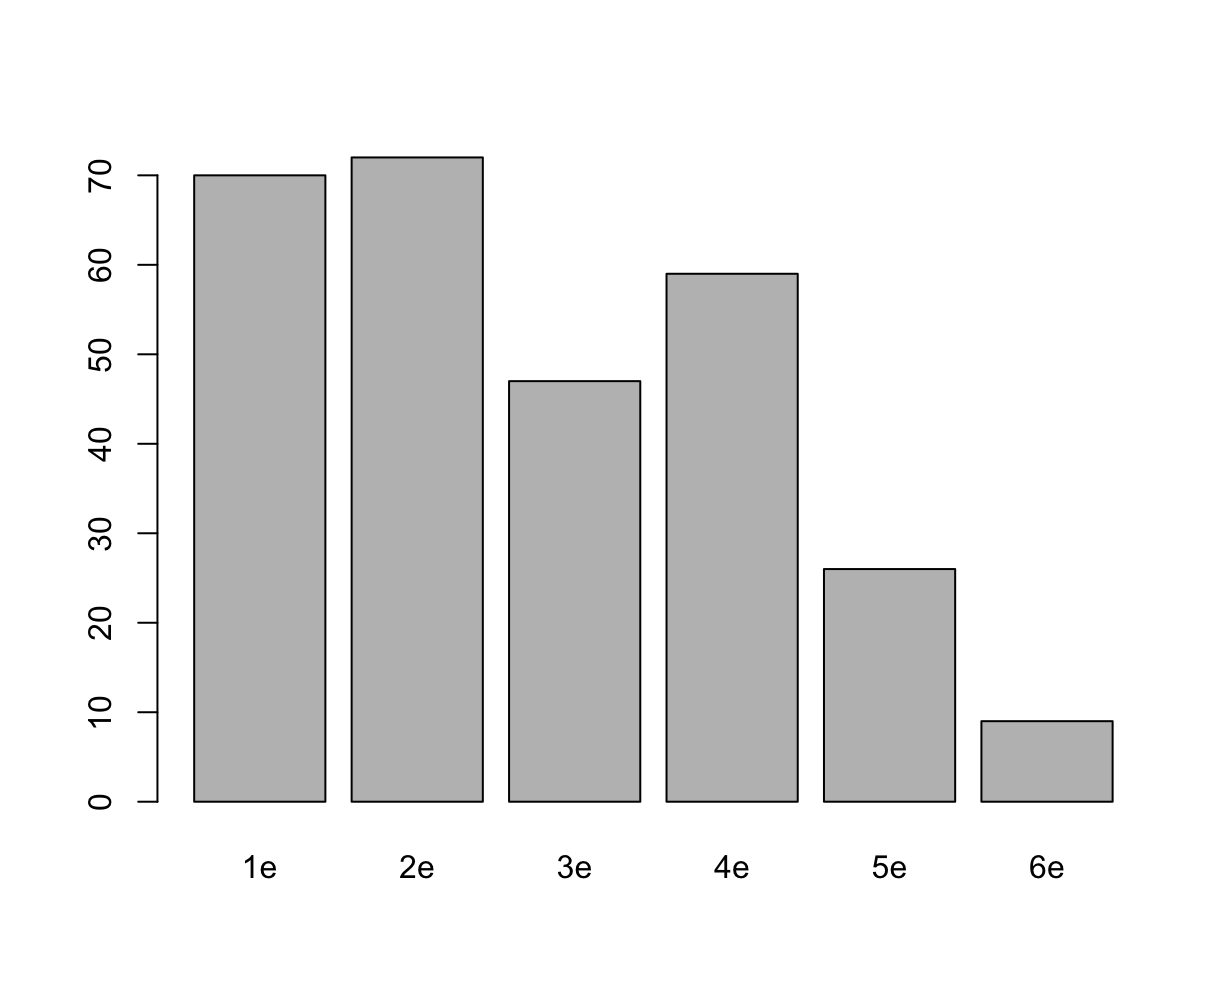
\includegraphics[width=0.5\textwidth]{Verdeling klassen.png}
    \caption{De verdeling van de respondenten tussen de jaren. (NA = 54)}
    \label{fig:verdeling}
    \end{figure}

You can see in figure {ref*{fig:distribution}} that most of the respondents are from undergrad. Year 5 and 6 are even poorly represented. Possible explanation is that the questionnaire was administered in March and these students were already mostly busy with exam preparations and their last day of school was approaching which may have made them feel less likely to benefit from this survey. Reproducing probably also plays less of a role in the exam year, although I have put lists of common signal words for the final French and German exams on the MemoryLab environment of the Metis Montessori Lyceum upon request. From year 4 students are again slightly more represented, which may be because the subjects of German, French and English in that year are very actively using MemoryLab in lessons.

\begin{figure}[h]
    \centering
    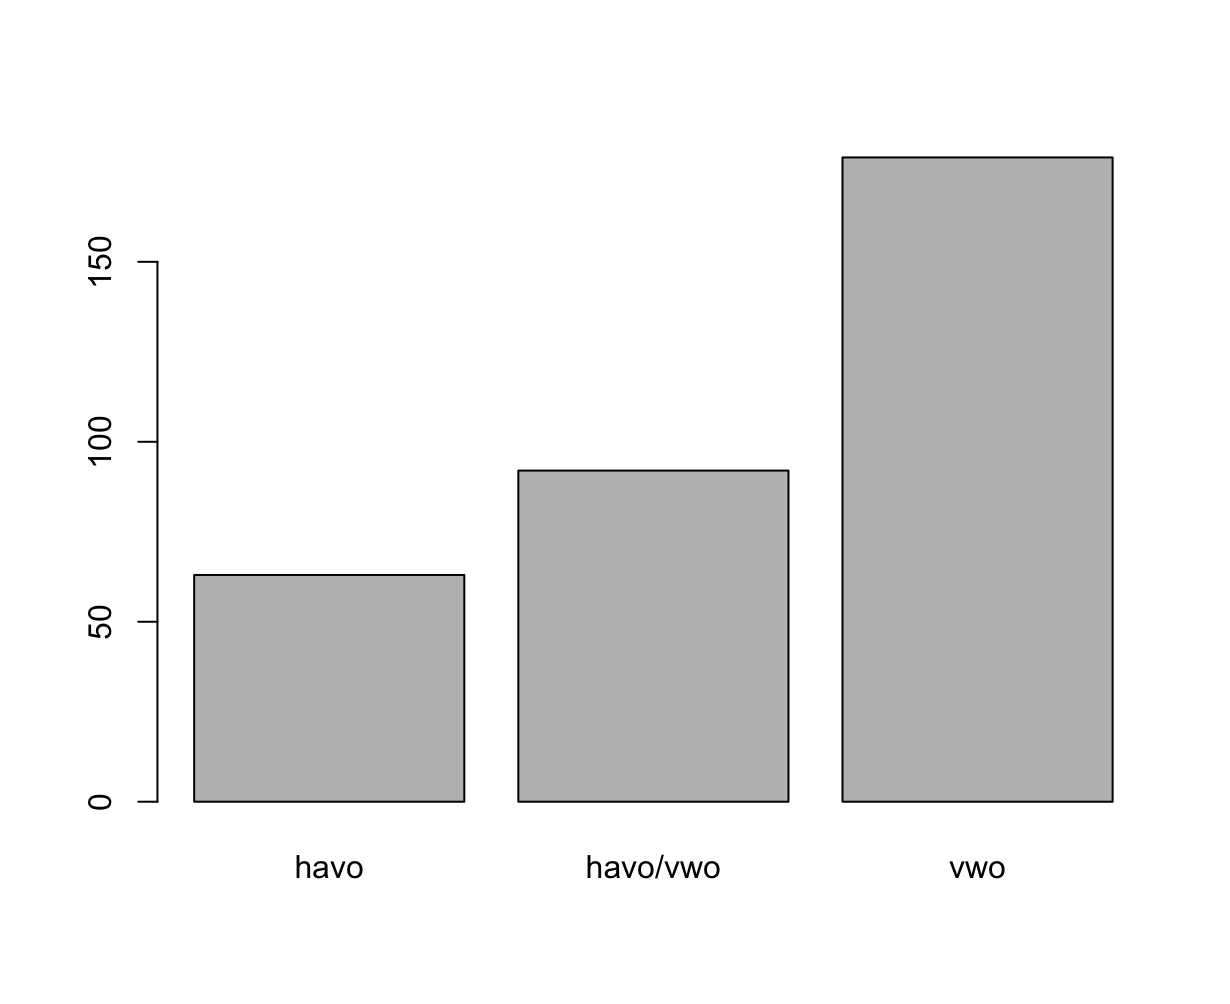
\includegraphics[width=0.5\textwidth]{niveau.png}
    \caption{Het huidige niveau van de respondenten. (NA = 3)}
    \label{fig:niveau}
    \end{figure}

Looking at level, we see in figure ref{fig:level} that the largest proportion of respondents do VWO level. This could indicate greater motivation and commitment among VWO students than HAVO students. But we have a 2-year bridge class HAVO/VWO in which there are also already many possibly HAVO students. We could also add the number of HAVO students to the HAVO/VWO then the ratio becomes much smaller (155 HAVO and 179 VWO).

\begin{figure}[h]
    \centering
    \includegraphics[width=0.5\textwidth]{kenJeMemoryLab.png}
    \caption{Gebruik je MemoryLab? (NA = 2)}
    \label{fig:kenJeMemoryLab}
    \end{figure}
When asked if respondents use MemoryLab, 285 respondents answered in the affirmative. Sixteen respondents no longer use it, 30 respondents do not use it, and 4 indicated that they have never heard of it. (See figure ref*{fig:kenJeMemoryLab}) If students did not use MemoryLab (anymore) respondents came directly to the closing questions. As a result, the direct questions about MemoryLab had around 285 responses.

Students had to respond to statements rated from 1 to 10, where 1=absolutely not and 10=absolutely yes. There are a few open-ended questions.

\subsection{prepared environment}
\begin{figure}
    \begin{tabular}{cc}
      \includegraphics[width=65mm]{12-MemoryLabIsDuidelijk.png} &   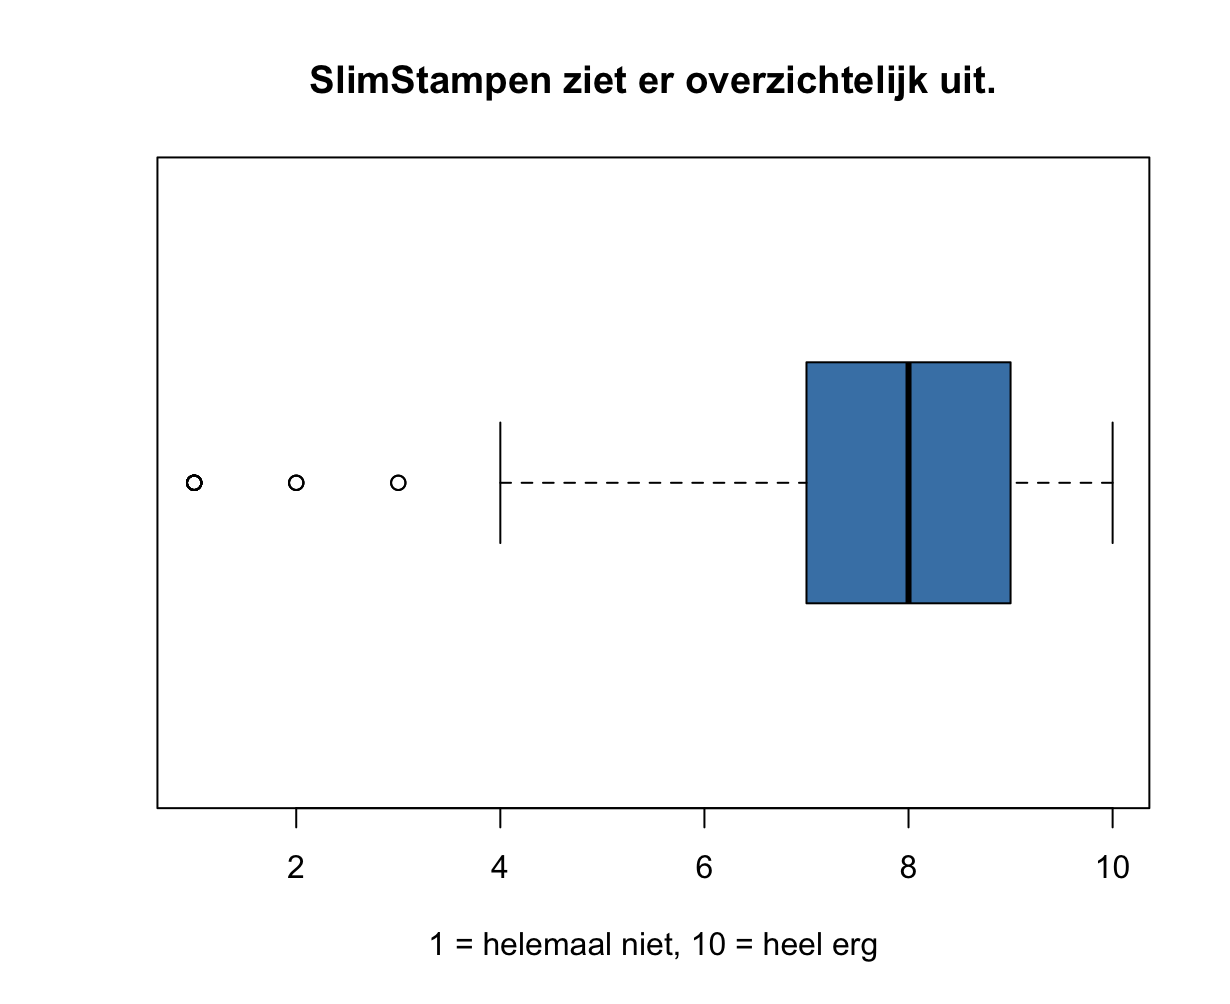
\includegraphics[width=65mm]{14-Overzichtelijk.png} \\
    (a)  $\overline{X}$ = 8.554, N=285, NA = 52 & (b) $\overline{X}$ = 7.663, N=285, NA = 52 \\[6pt]
    \end{tabular}
    \caption{indicatoren voor de voorbereide omgeving}
    \label{fig:omgeving}
    \end{figure}

The prepared environment is a broad term for Montessori. Not only should the physical classroom and educational materials be in order and meet certain requirements, but the teacher is also part of the prepared environment. So MemoryLab, as an educational material, is only a small part of the prepared environment. Thus, this study addresses only a small part of the preparation. With the use of MemoryLab, the teacher makes sure the material is ready. The students are free to grab it themselves and can work with this material independently at those times when they want to work with it themselves. They can check their own mistakes so completely independent of the teacher they can get to work.
The results show that MemoryLab as a material looks clear and students know what to do there. When asked whether it is clear what to do with MemoryLab (see Figure ref*{fig:environment}(a)), you can see that the first quartile is already at eight, the second quartile even at ten. Students know what this material is for and can use it. Also, when asked if MemoryLab is clear, most students are extremely positive (see Figure ref*{fig:environment}(b)). In conclusion; students are positive about the material per se.

\subsection{normalization}
\begin{figure}
    \begin{tabular}{cc}
      \includegraphics[width=65mm]{11-AlsIkNietWeetGaMemoryLab.png} &   \includegraphics[width=65mm]{13-ConcentratieBijMemoryLab.png} \\
    (a)  $\overline{X}$ = 5.568, N=285, NA = 52 & (b) $\overline{X}$ = 7.616, N=284, NA = 53 \\[6pt]
     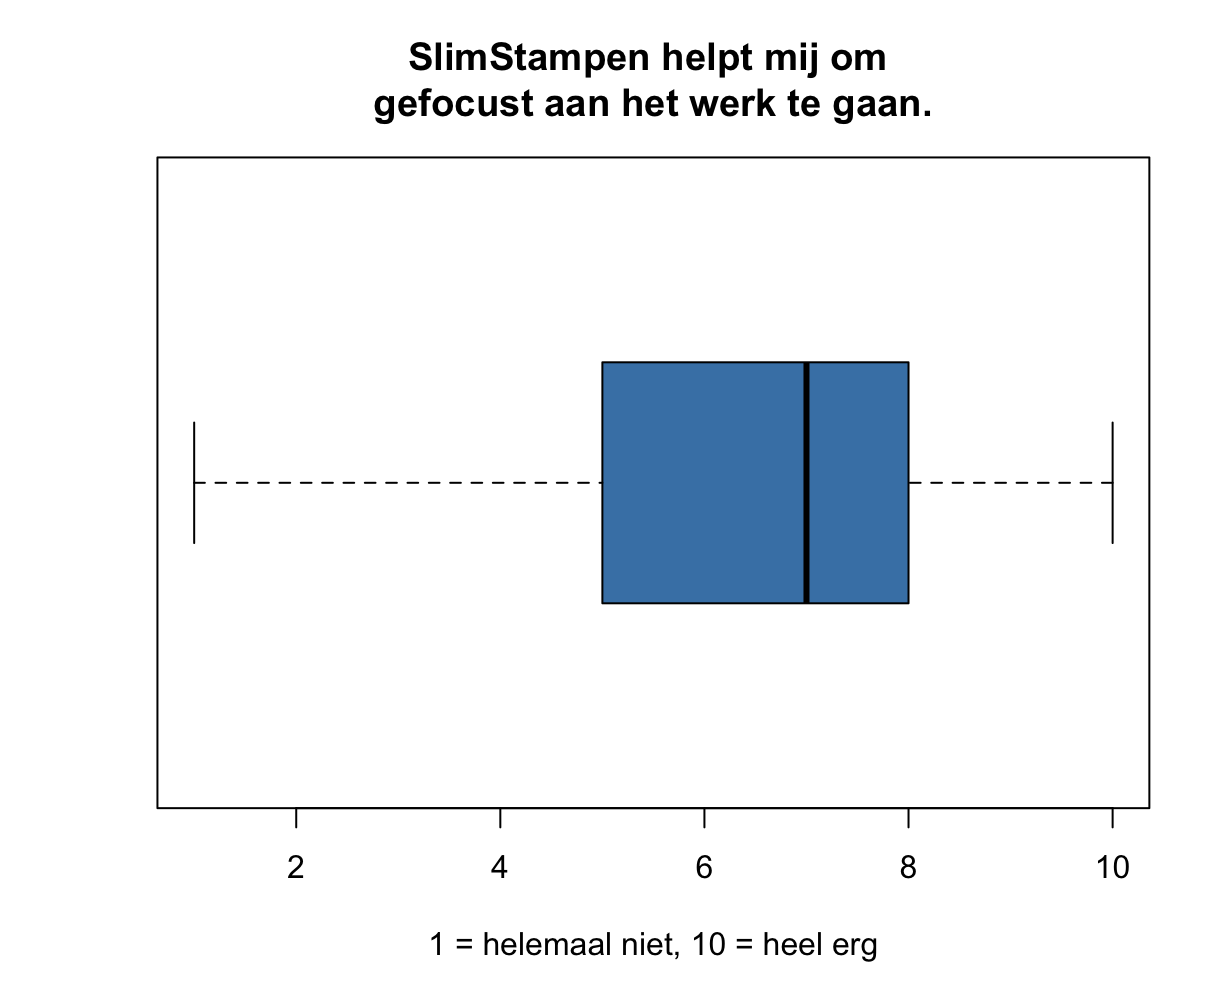
\includegraphics[width=65mm]{17-GefocustAanHetWerk.png} &   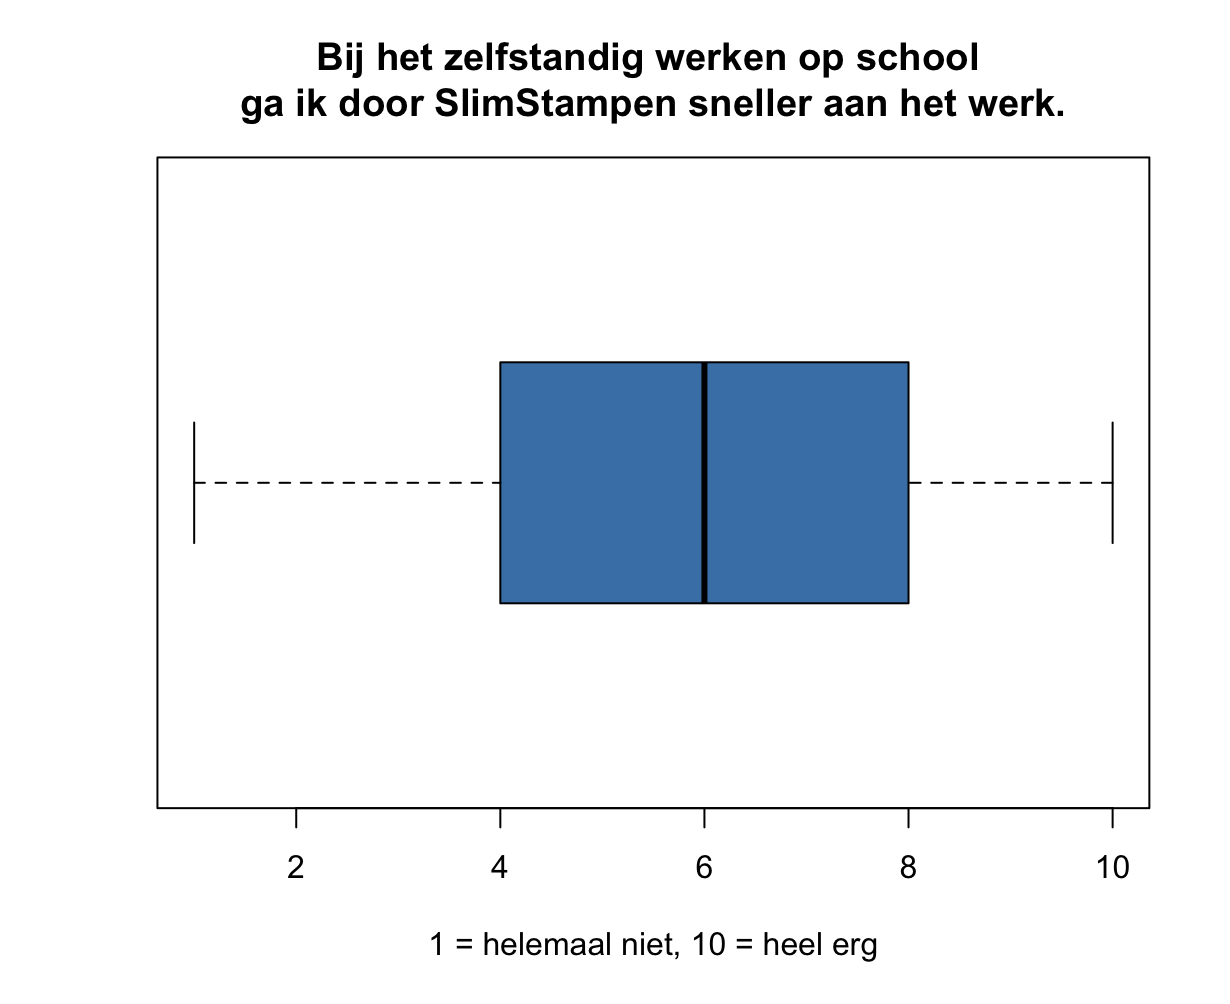
\includegraphics[width=65mm]{18-SnellerAanHetWerk.png} \\
    (c) $\overline{X}$ = 6.553, N=284, NA = 53 & (d) $\overline{X}$ = 6.018, N=284, NA = 53 \\[6pt]
    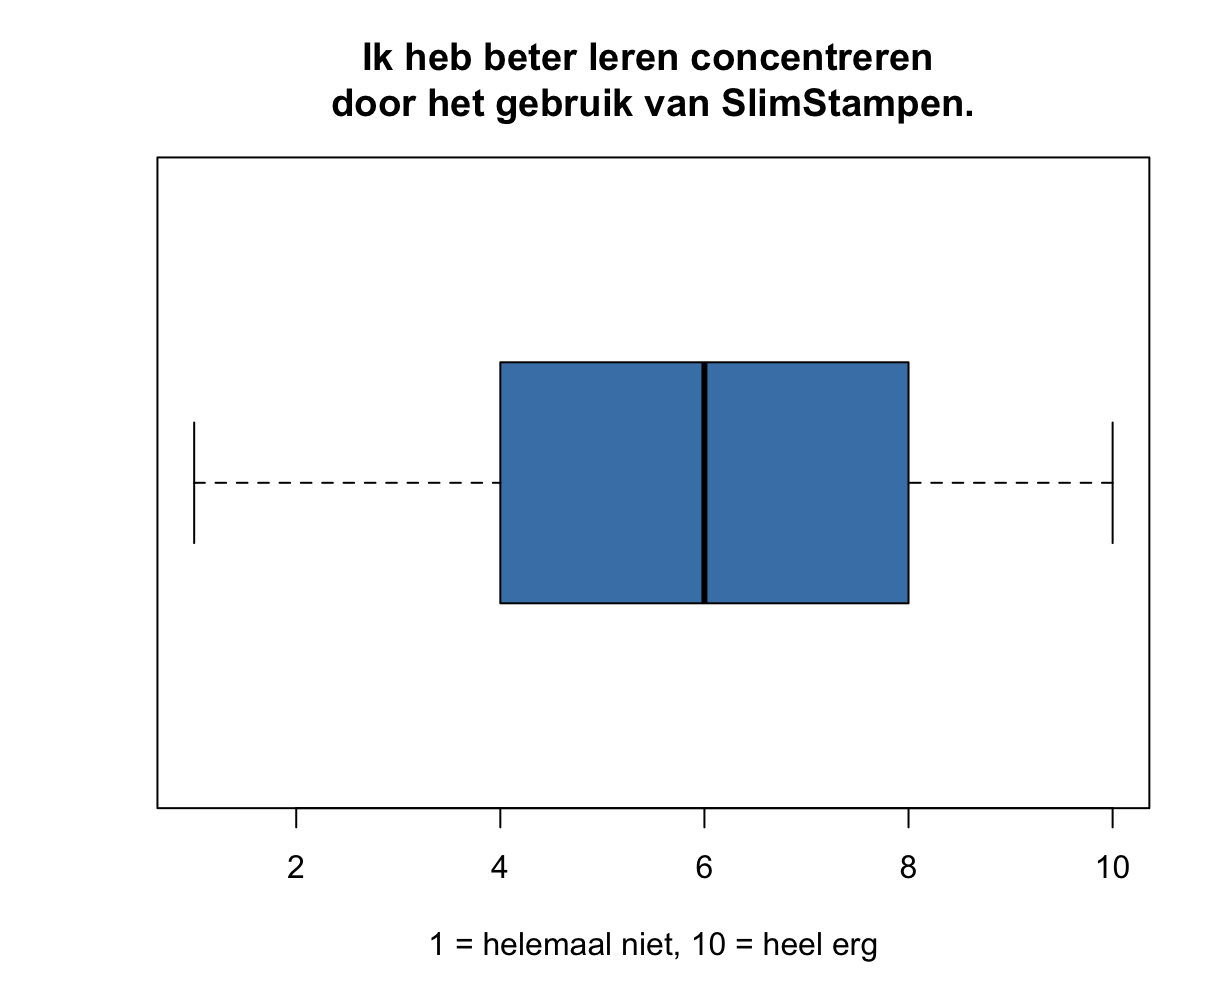
\includegraphics[width=65mm]{28-BeterLerenConcentreren.png} & 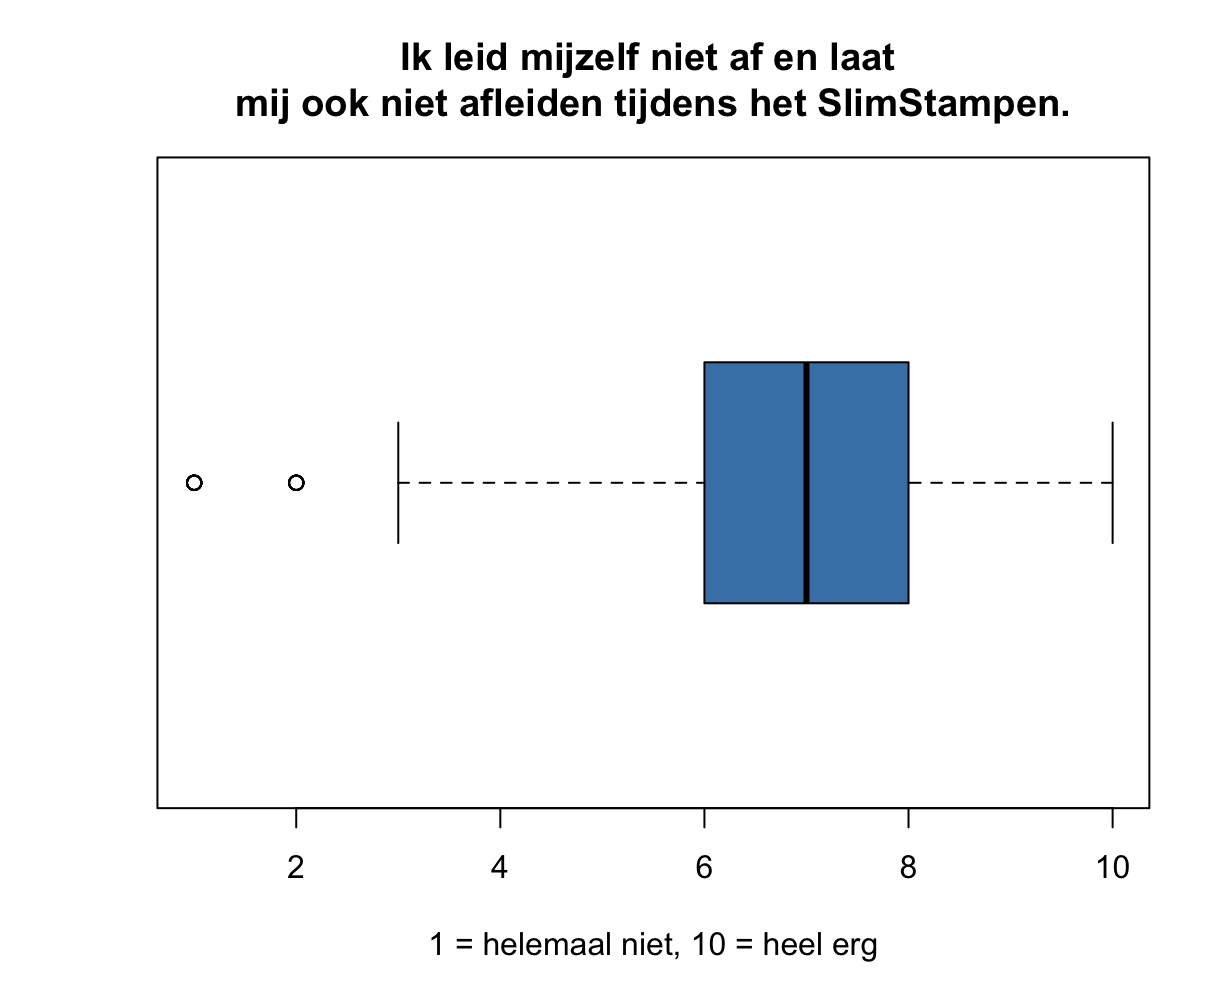
\includegraphics[width=65mm]{images/15-LaatNietAfleiden.png}\\
    (e) $\overline{X}$ = 5.879, N=281, NA = 56 & (f) $\overline{X}$ = 6.705, N=285, NA = 52  
    \end{tabular}
    \caption{indicatoren voor betere normalisatie}
    \label{fig:normalisatie}
    \end{figure}
Learner normalization is difficult to measure and can be interpreted in many ways. Mainly through observation, you can observe whether a learner is "normalized. A learner can begin work independently and can bring himself into deeper concentration without the need for the teacher. Normalization touches the learner's task acceptance. Does MemoryLab help concentration and does a student get to work faster because of MemoryLab? The answers to these questions give an indication of student normalization.

Figure ref*{fig:normalization}(a) shows that many students do not automatically reach for MemoryLab when they are momentarily unsure of what to do. My idea was that MemoryLab could also be used as an alternative to other work. If the student does not know what to do for a while that it would then easily go to MemoryLab. This hypothesis is not convincingly positive.
Students are overwhelmingly positive about the concentration they achieve when working with MemoryLab {ref*{fig:normalization}(b). This is kind of necessary because the learning algorithm takes reaction time into account.

MemoryLab helps many students get to work focused. This fits well with what Maria Montessori saw as standardization. This is also my experience during my observation; when students start in the class hour with MemoryLab they quickly get into "learning mode" (see figure ref*{fig:normalization}(c)).

Whether MemoryLab helps students get to work faster during class are fairly neutral. I have some idea, but this is not strongly reflected in the data (see figure ref*{fig:normalization}(d)).
I had hoped that students would experience and learn the importance of concentration with the use of MemoryLab. This is not readily apparent from figure {ref*{fig:normalization}(e). In any case, they indicate that they do not immediately learn to concentrate better.
Figure Êref*{fig:normalization}(f) shows that students are not easily distracted when using MemoryLab, nor do they distract themselves. It is plausible (see also Figure ref*{fig:normalization}(b)) that they unconsciously reach the state of deep concentration while working with MemoryLab.

\subsection{Motivation}
\begin{figure}
    \begin{tabular}{cc}
      \includegraphics[width=65mm]{images/16-TwijfelGaIkMemoryLab.png} &   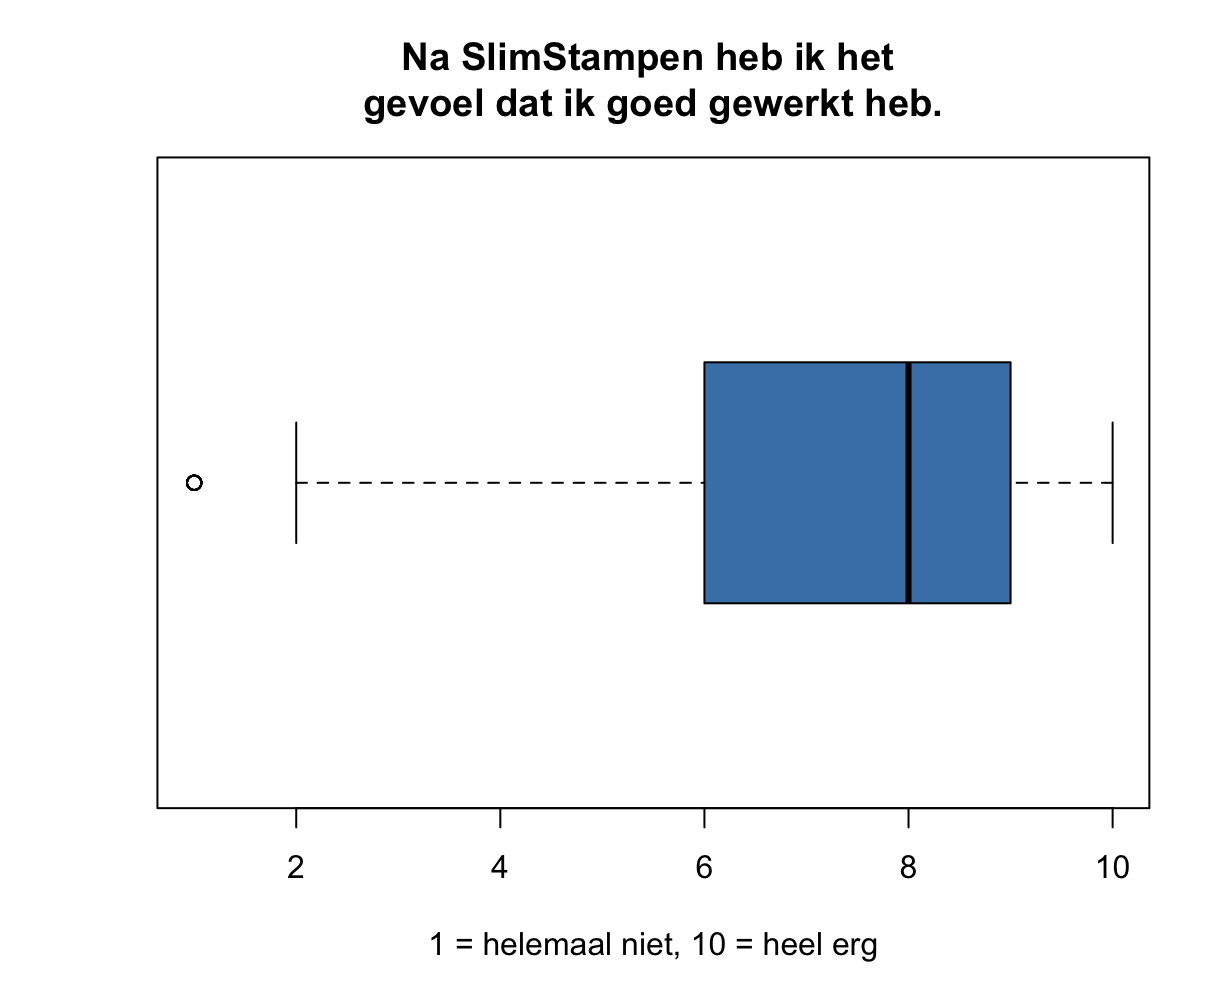
\includegraphics[width=65mm]{images/19-GevoelGoedGewerkt.png} \\
    (a) $\overline{X}$ = 5.855, N=283, NA = 54   & (b) $\overline{X}$ = 7.34, N=285, NA = 52  \\[6pt]
     \includegraphics[width=65mm]{images/20-MemoryLabLeukerDanRijtjes.png} &   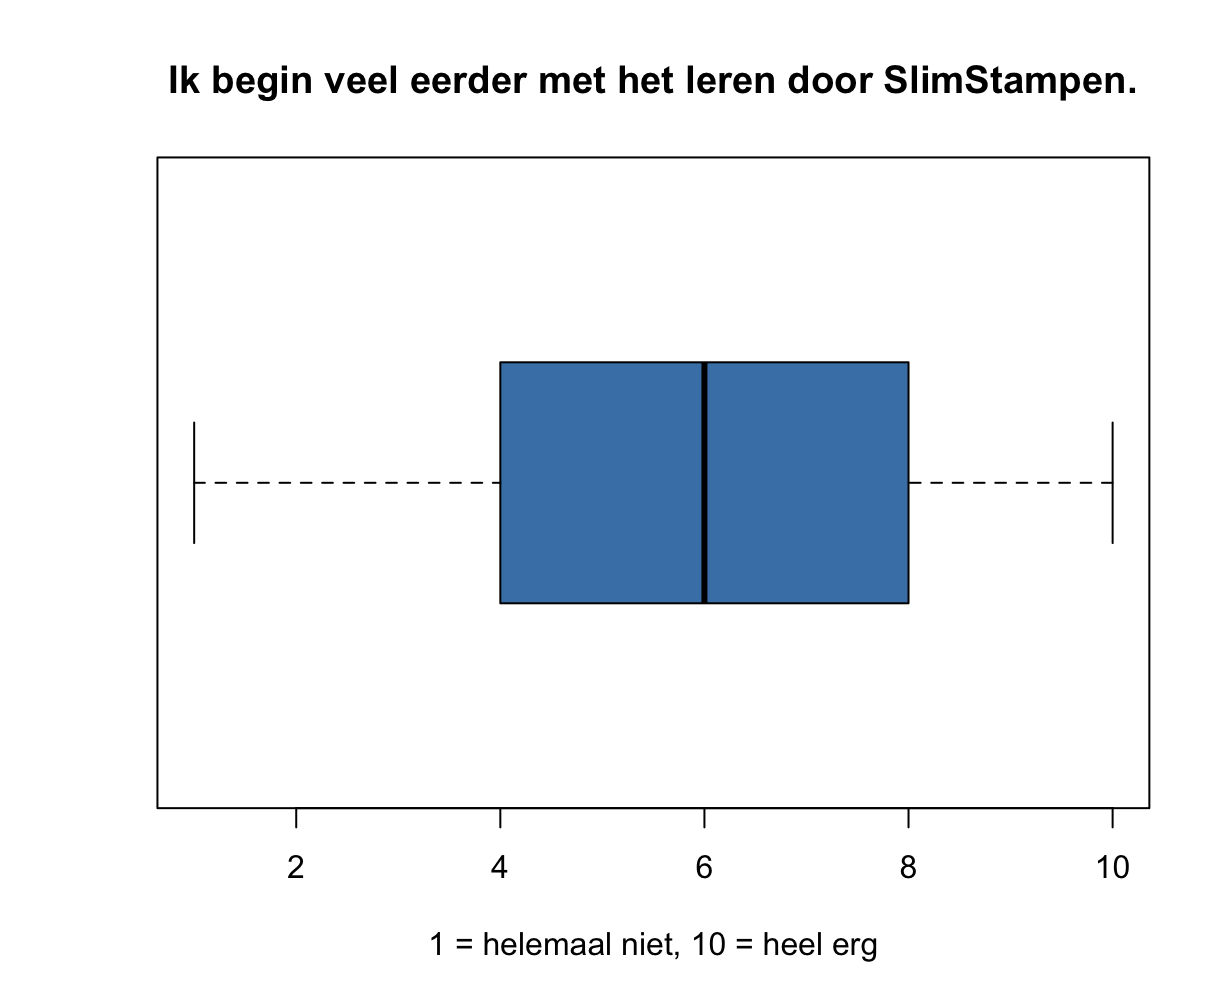
\includegraphics[width=65mm]{images/21-BeginEerder.png} \\
    (c) $\overline{X}$ = 7.818, N=280, NA = 57  & (d) $\overline{X}$ = 6.163, N=283, NA = 54  \\[6pt]
    \multicolumn{2}{c}{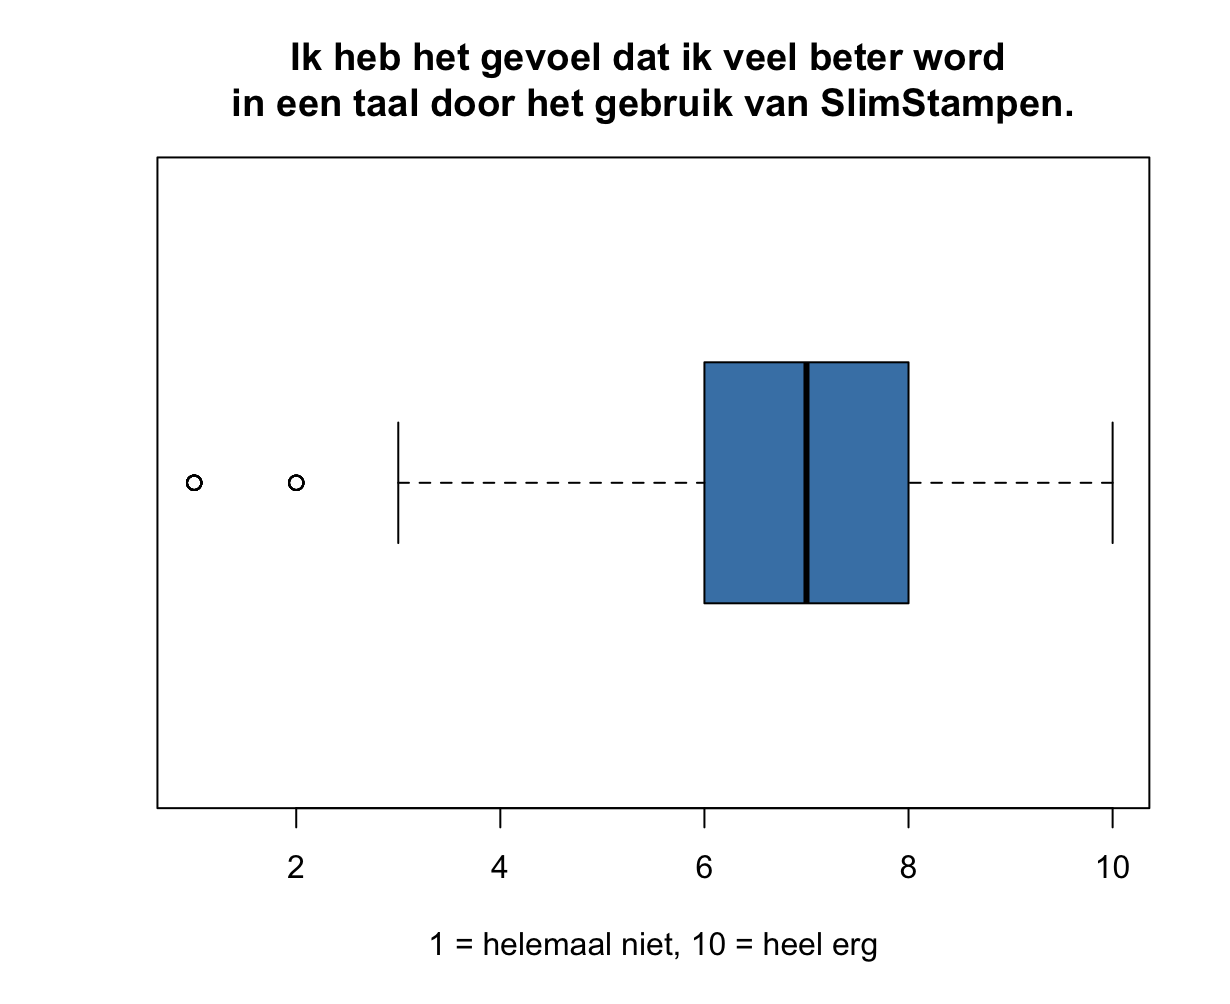
\includegraphics[width=65mm]{23-BeterInTaal.png} }\\
    \multicolumn{2}{c}{(e) $\overline{X}$ = 6.852, N=283, NA = 54}
    \end{tabular}
    \caption{indicatoren voor hogere motivatie}
    \label{fig:motivatie}
    \end{figure}

Maria Montessori assumed the intrinsic motivation of the learner. Children have an absorbing mind and want to learn. Teenagers are past this sensitive period for absorbing knowledge. The development of personality and as an individual is more important at this stage. Nevertheless, imparting knowledge is one of the goals of education, including secondary education. This succeeds only if the student is somewhat motivated, intrinsically or extrinsically. According to Deci and Ryan's self-determination theory, students have three basic needs: autonomy, competence and connectedness. If these needs are met, the learner is a lot more likely to be motivated.

Making sense of something is a form of intrinsic motivation. Even if it is sometimes a choice between two evils for a learner. MemoryLab is not that difficult in the sense that it is simply ''stamping.'' No higher thinking skills are addressed. Mind zero and get to work. I was curious if students would see MemoryLab in the same way. Not keen on higher thinking skills, but energized enough to MemoryLab. This hypothesis is not shared by all students. They are slightly positive about this, but a large proportion are also not (see figure ref*{fig:motivation}(a)).
Feeling positive after working provides motivation for next time. Does learning with MemoryLab give you a positive feeling afterwards? This is something most students agree on. Figure ref*{fig:motivation}(b) clearly shows that many students feel they worked well after practicing with MemoryLab.

Memorizing words for a test happens almost in every school. It is simply cramming knowledge. Not always fun, but necessary to learn a new language, for example. Most students report that learning facts with MemoryLab is much more fun than learning rows. In figure ref*{fig:motivation}(c) you can see that almost all students are positive to very positive about this.

When asked whether students start learning much earlier because of MemoryLab, students are fairly normally distributed. The mean is a 6.163 just positive (see figure ref*{fig:motivation}(d)). My idea with this question was that motivated students are more likely to start a task by themselves. With MemoryLab, you are required to learn for at least three days (per day you can get a mastery crown). So it may be that students will start earlier for that reason alone.

In figure ref*{fig:motivation}(e), you can see that many students generally feel that they are getting better at a language by using MemoryLab. This will most likely make them feel more confident about learning a language and probably thus more motivated.

\begin{figure}
    \begin{tabular}{cc}
      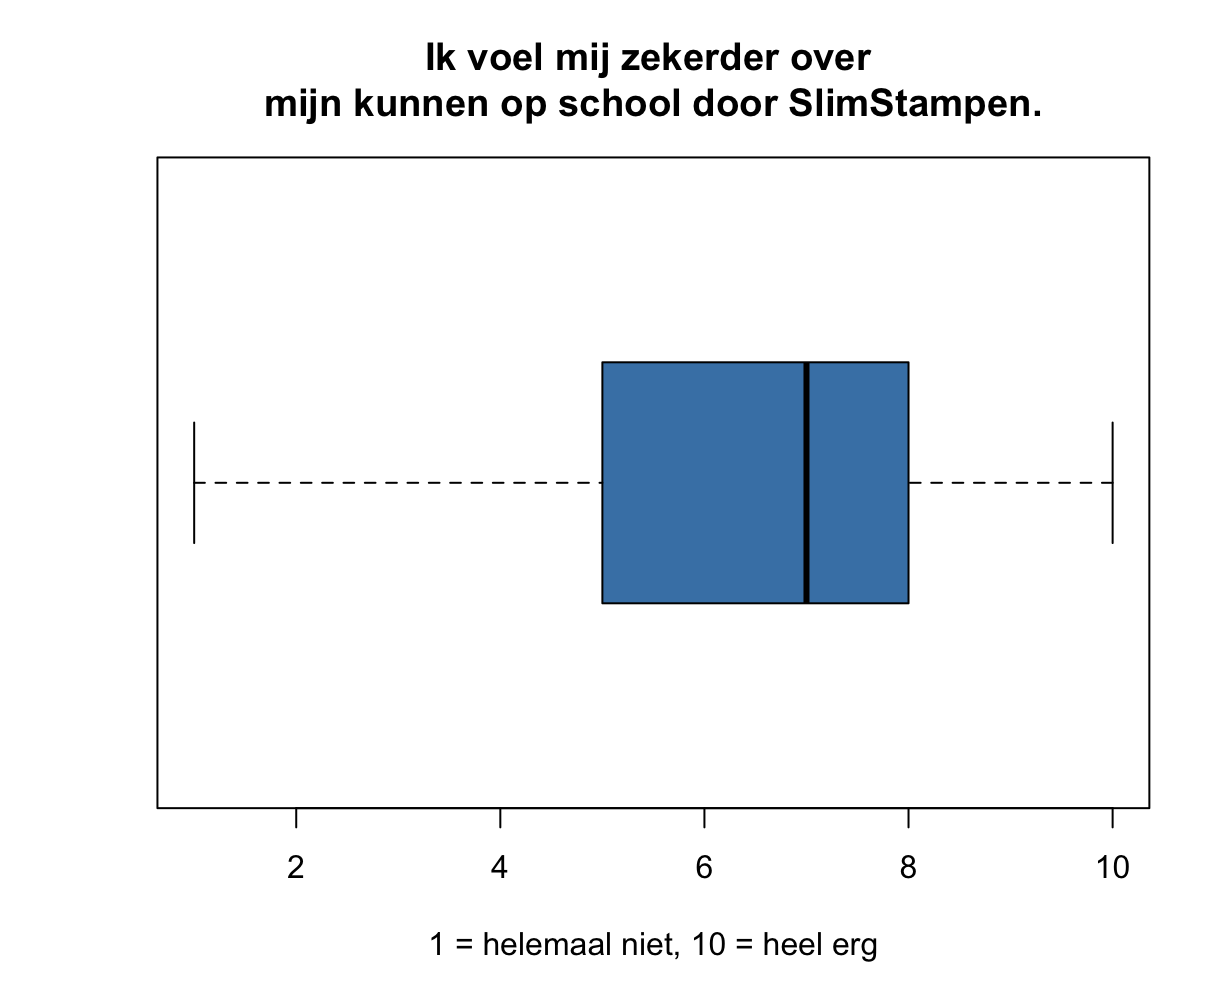
\includegraphics[width=65mm]{images/24-VoelZekerder.png} &   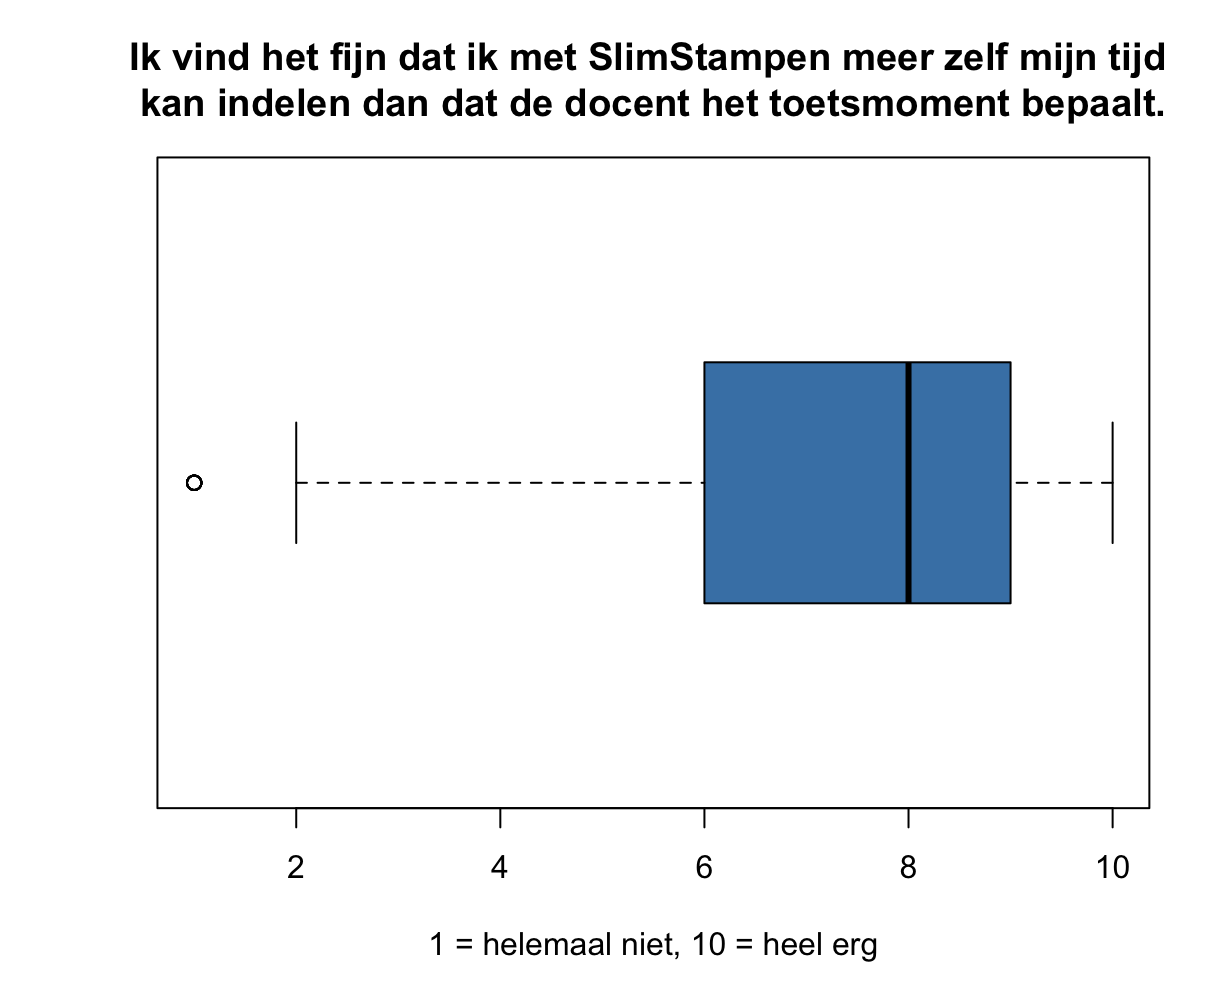
\includegraphics[width=65mm]{images/27-ZelfTijdIndelen.png} \\
    (a) $\overline{X}$ = 6.246, N=281, NA = 56   & (b) $\overline{X}$ = 7.241, N=282, NA = 55  \\[6pt]
     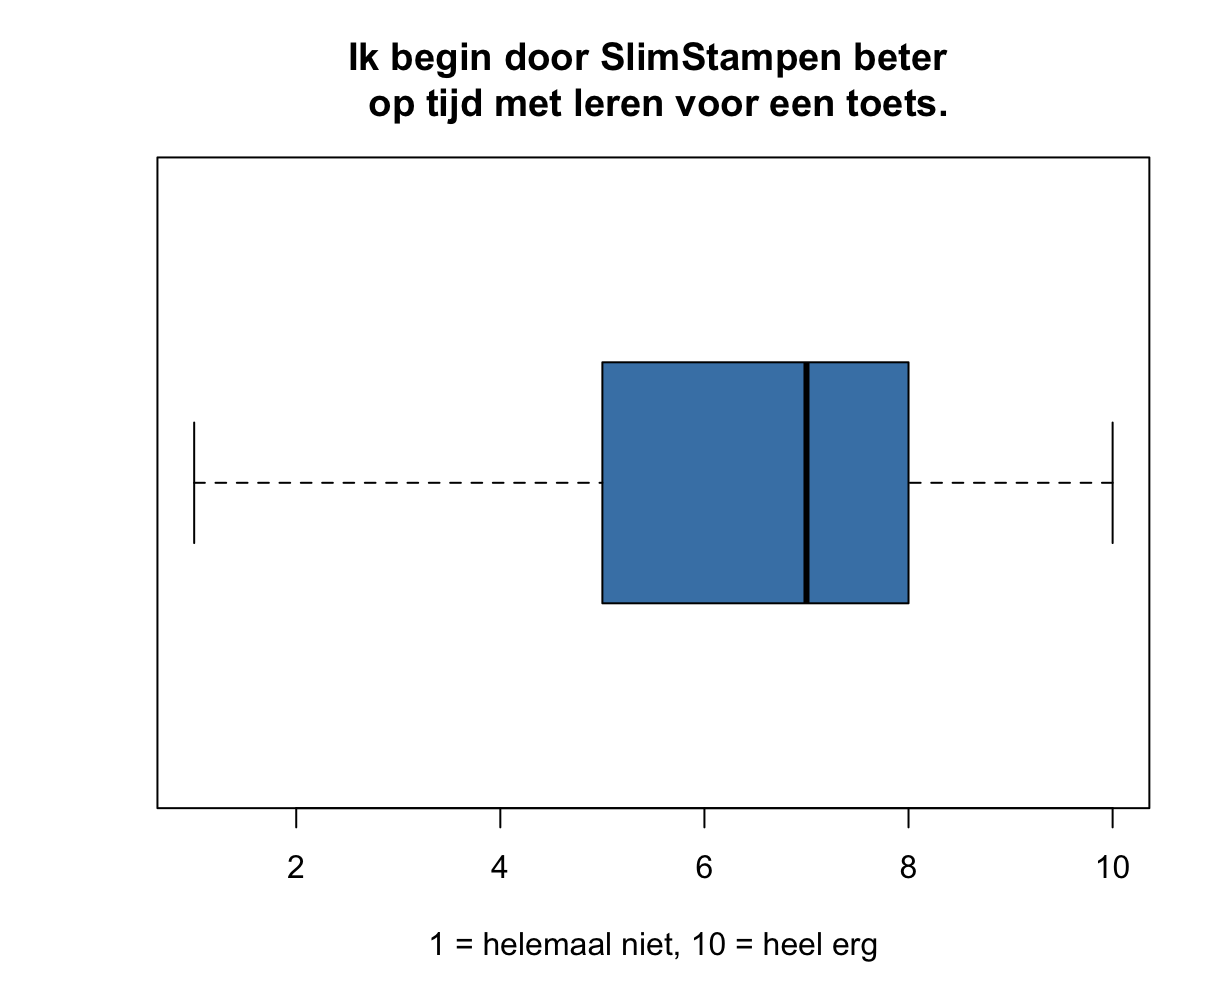
\includegraphics[width=65mm]{images/29-OpTijdBeginnenLeren.png} &   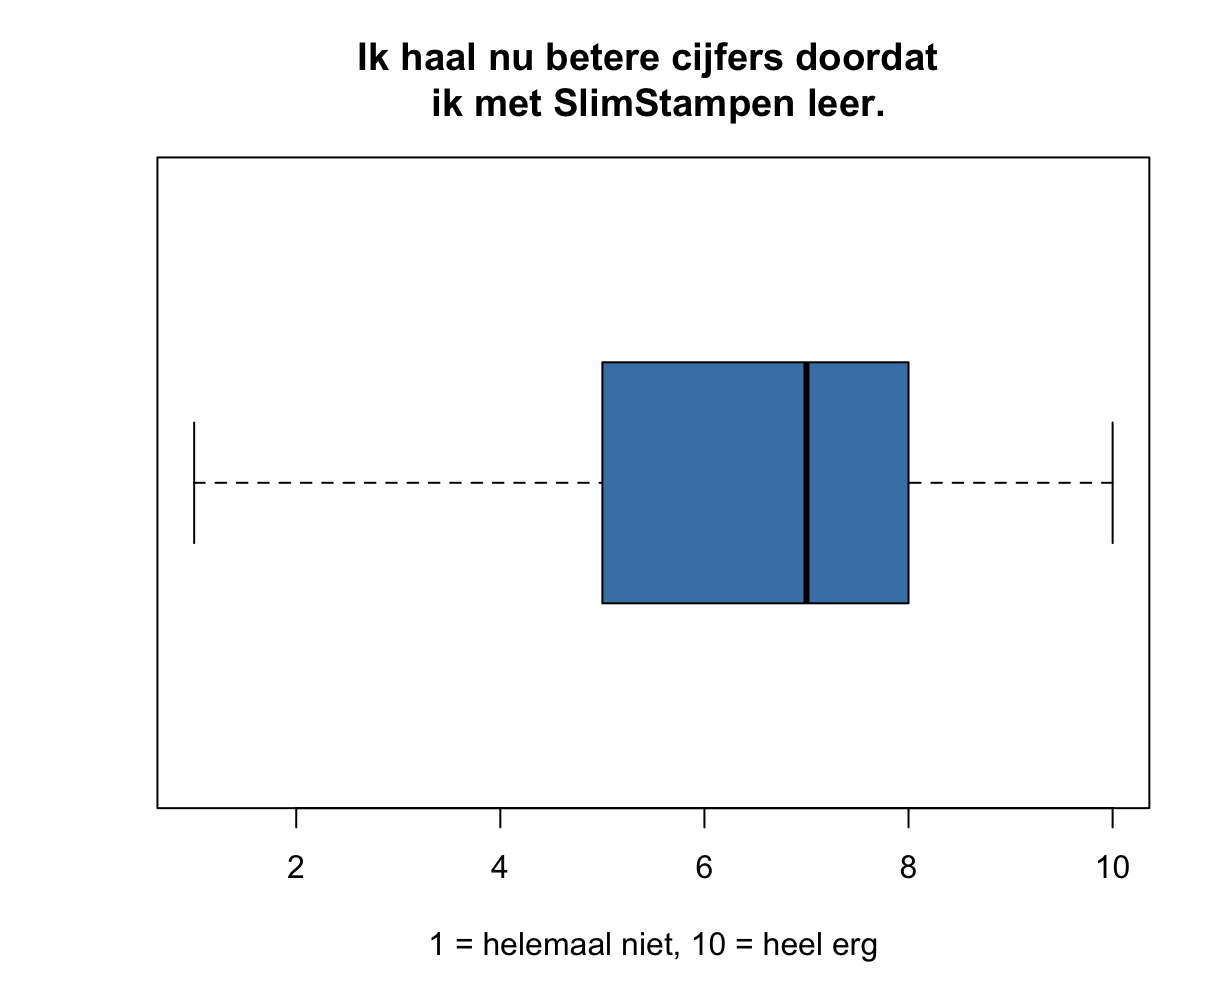
\includegraphics[width=65mm]{images/30-BetereCijfers.png} \\
    (c) $\overline{X}$ = 6.192, N=281, NA = 56  & (d) $\overline{X}$ = 6.529, N=280, NA = 57  \\[6pt]
    \end{tabular}
    \caption{indicatoren voor hogere motivatie}
    \label{fig:motivatie2}
    \end{figure}

Students who feel competent are generally more motivated for school. When asked whether students feel
more confident at school about their competence through the use of MemoryLab, students are generally quite positive
(see figure ref*{fig:motivation2}(a)). When asked if they like the fact that the use allows them to schedule more of their own time instead of the teacher determining the test time, by far the majority of students are positive. Here we are addressing students' autonomy. You can see in figure ref*{fig:motivation2}(b) that only a few students respond negatively to this. A few outliers of learners who are even outright negative. These could be students who ''just filled out'' something, but I don't have that idea. I will come back to that in Section 6.6. Looking at Deci and Ryan's self-determination theory, it is important that students experience autonomy and competence. These are two of the three basic needs of learners. These are addressed through the use of MemoryLab.

The question ''I am starting to learn better on time for a test because of MemoryLab'' from figure ref*{fig:motivation2}(c) is very similar to the question from figure ref*{fig:motivation}(d). I have focused this question a bit more on specifically learning for a test. Here, students also generally answer slightly more positively than the more general question about starting earlier. Interestingly, the distribution of the next question about getting higher grades with MemoryLab is very similar to starting to learn the test earlier. The mean is even slightly higher as you can see in figure ref*{fig:motivation2}(d).

As a conclusion, MemoryLab has a positive impact on student motivation. Students feel more confident about their abilities, like the fact that they have more autonomy, and start learning earlier for a test. All of this leads to better grades.

\subsection{Learning Strategies}
\begin{figure}
    \begin{tabular}{cc}
      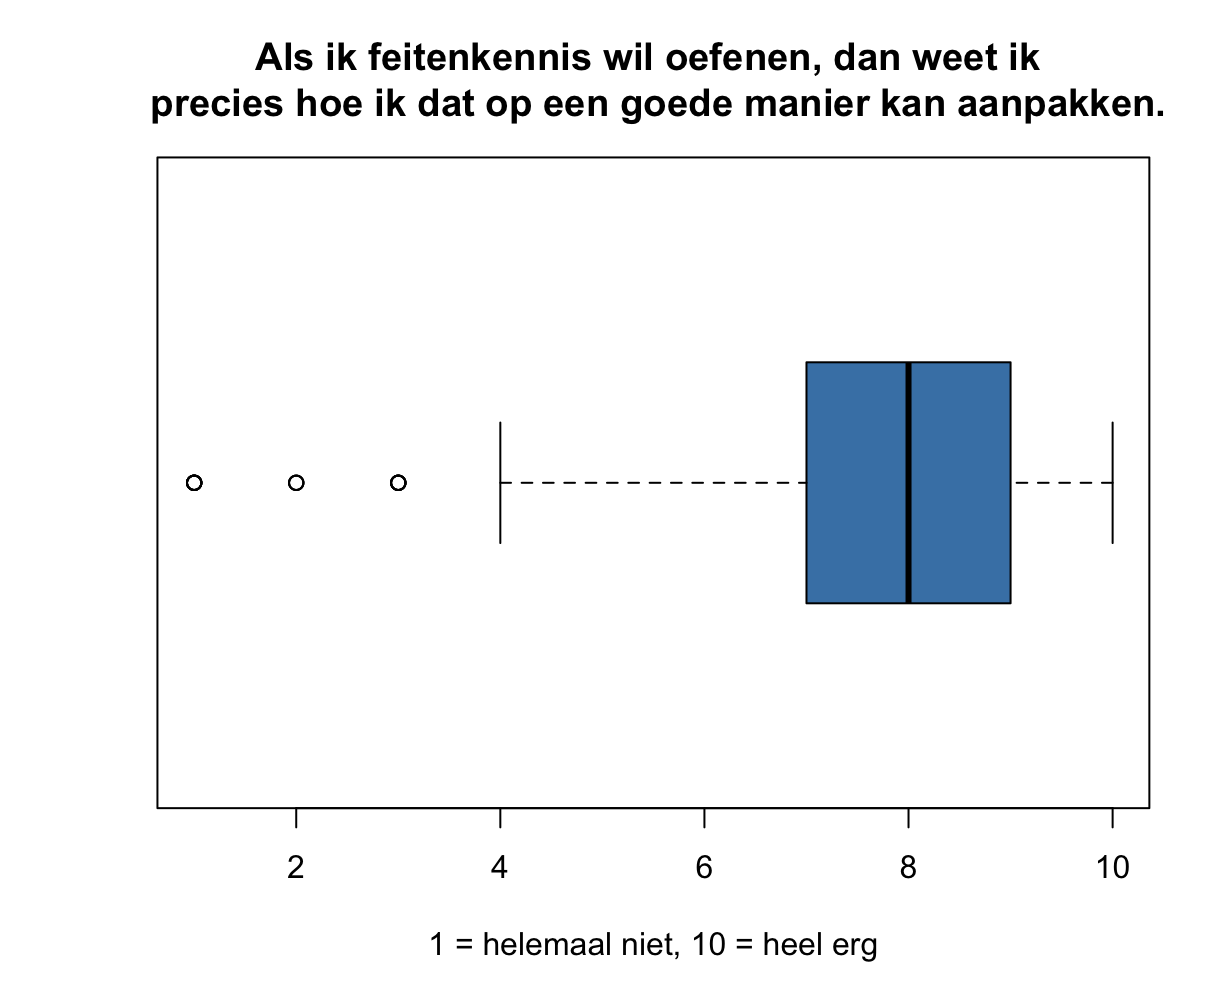
\includegraphics[width=65mm]{04-WeetAanpakken.png} &   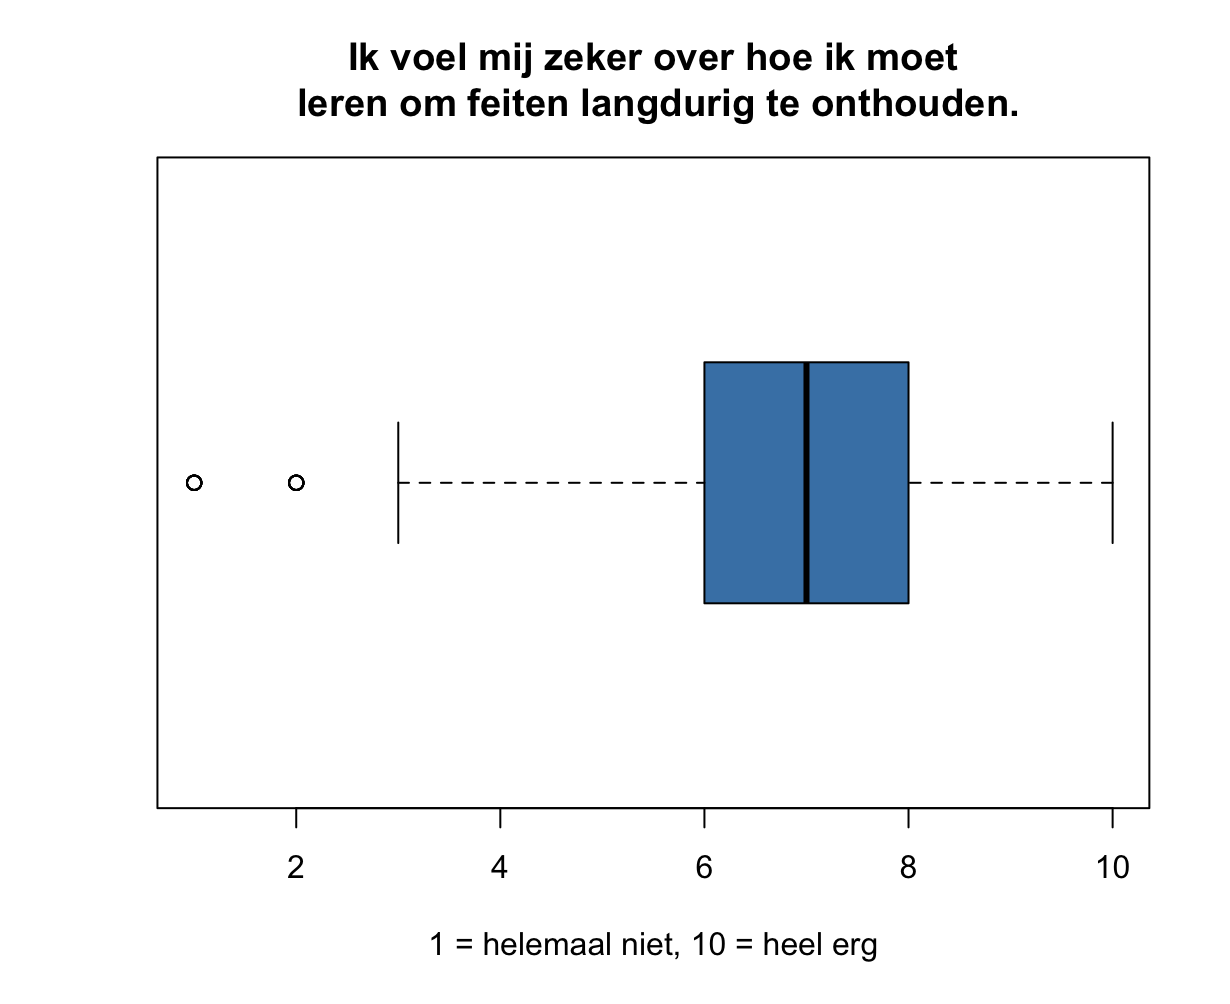
\includegraphics[width=65mm]{06-zekerOverOnthouden.png} \\
    (a)  $\overline{X}$ = 7.634, N=333, NA = 4 & (b) $\overline{X}$ =  6.83, N=335, NA = 2 \\[6pt]
    \multicolumn{2}{c}{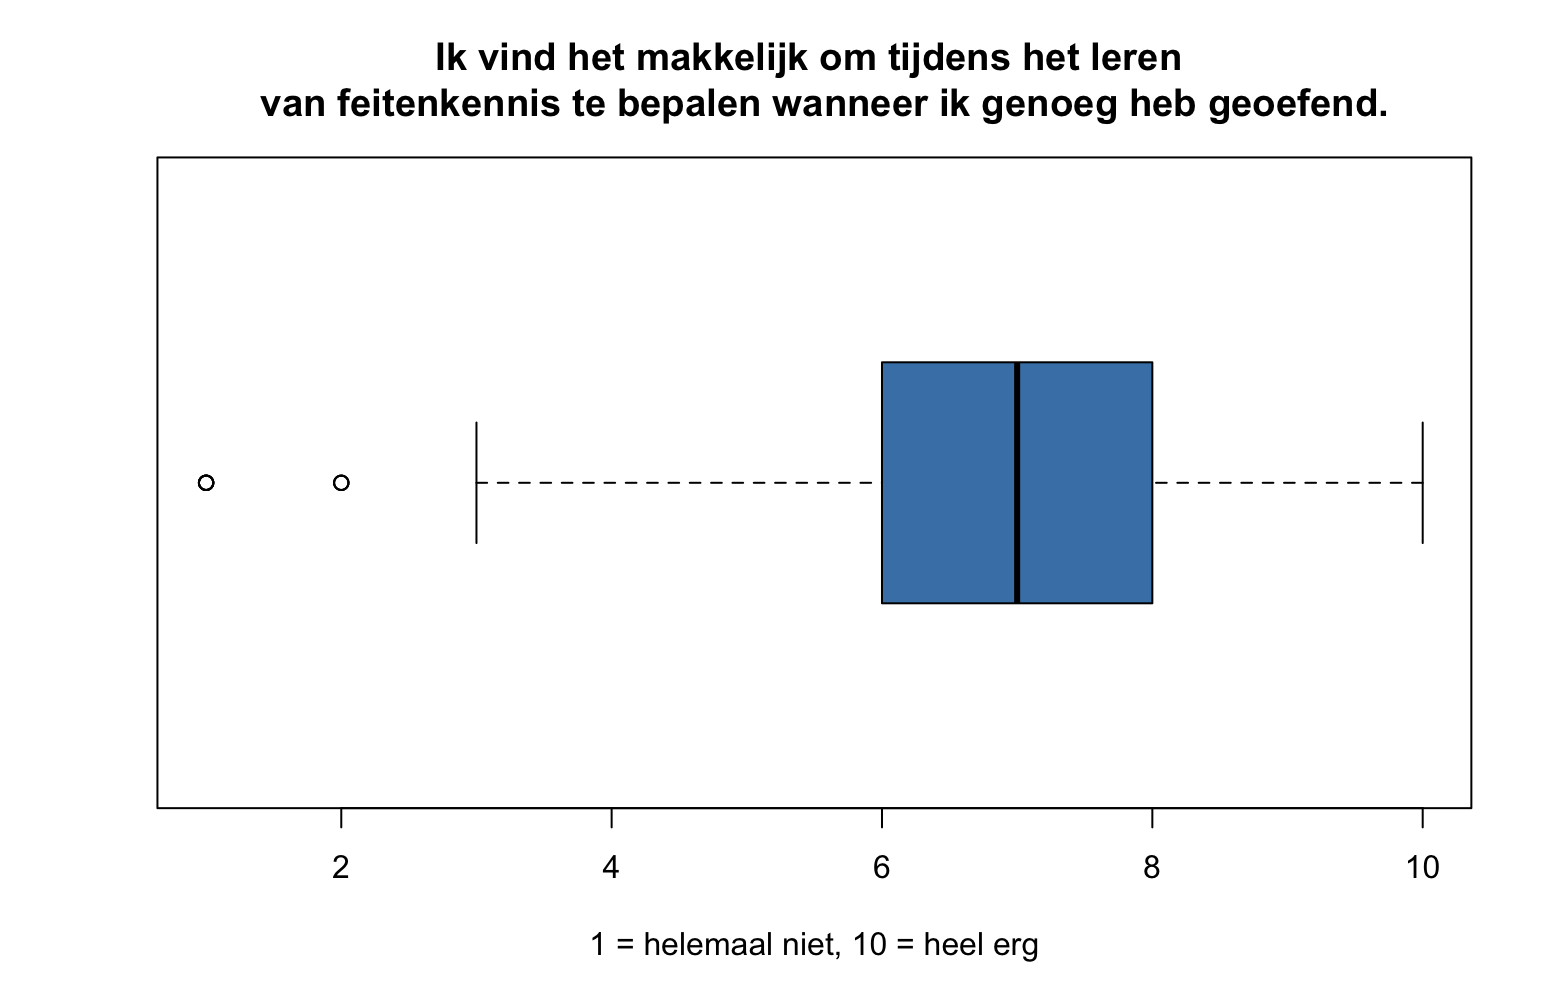
\includegraphics[width=65mm]{05-bepalenGenoegGeoefend.png} }\\
    \multicolumn{2}{c}{(e) $\overline{X}$ = 7.224, N=331, NA = 6}
    \end{tabular}
    \caption{kennis over leerstrategieën}
    \label{fig:leerstrategie}
    \end{figure}

    \begin{figure}
        \begin{tabular}{cc}
          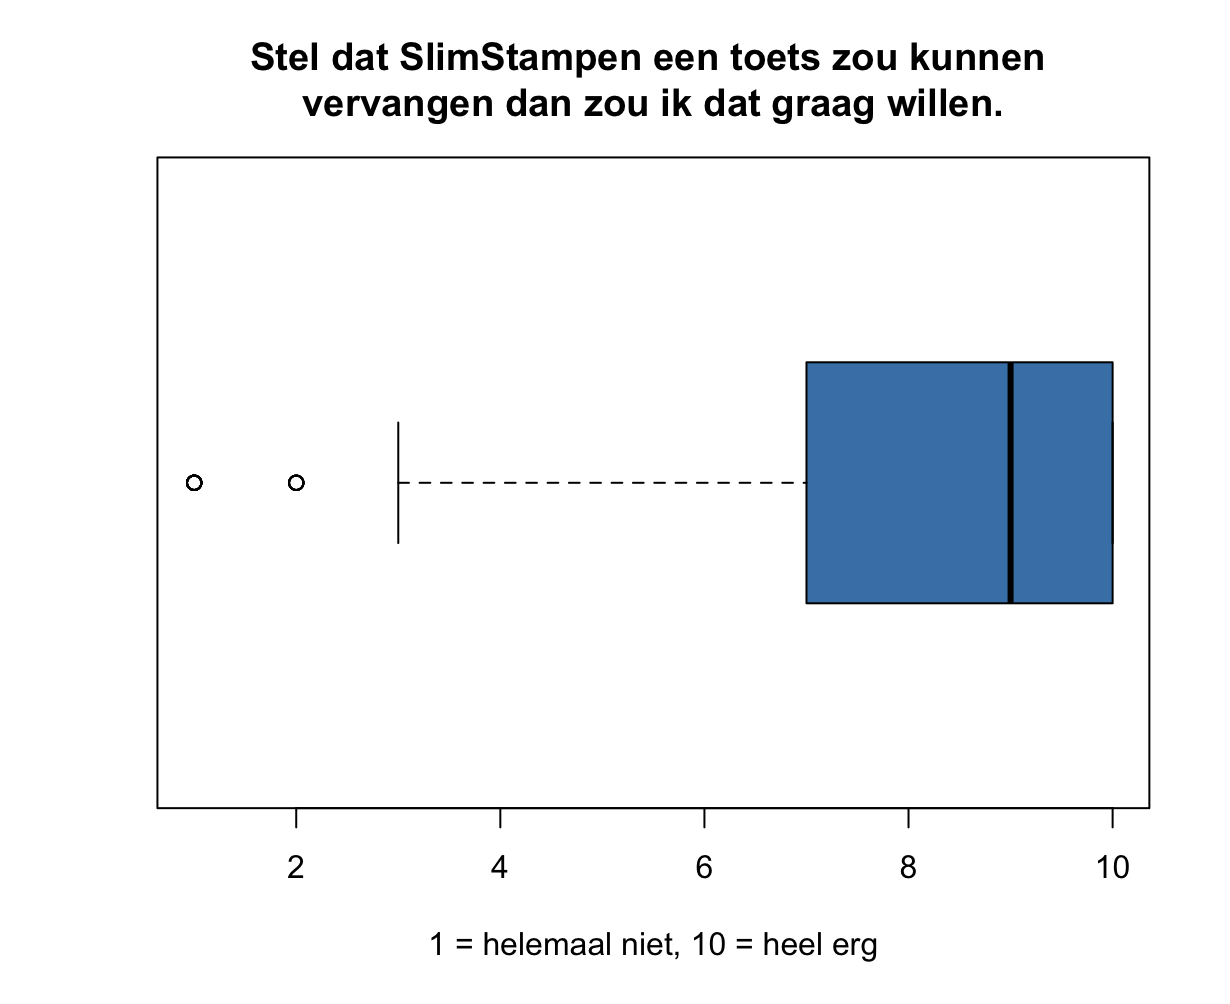
\includegraphics[width=65mm]{25-ToetsVervangen.png} &   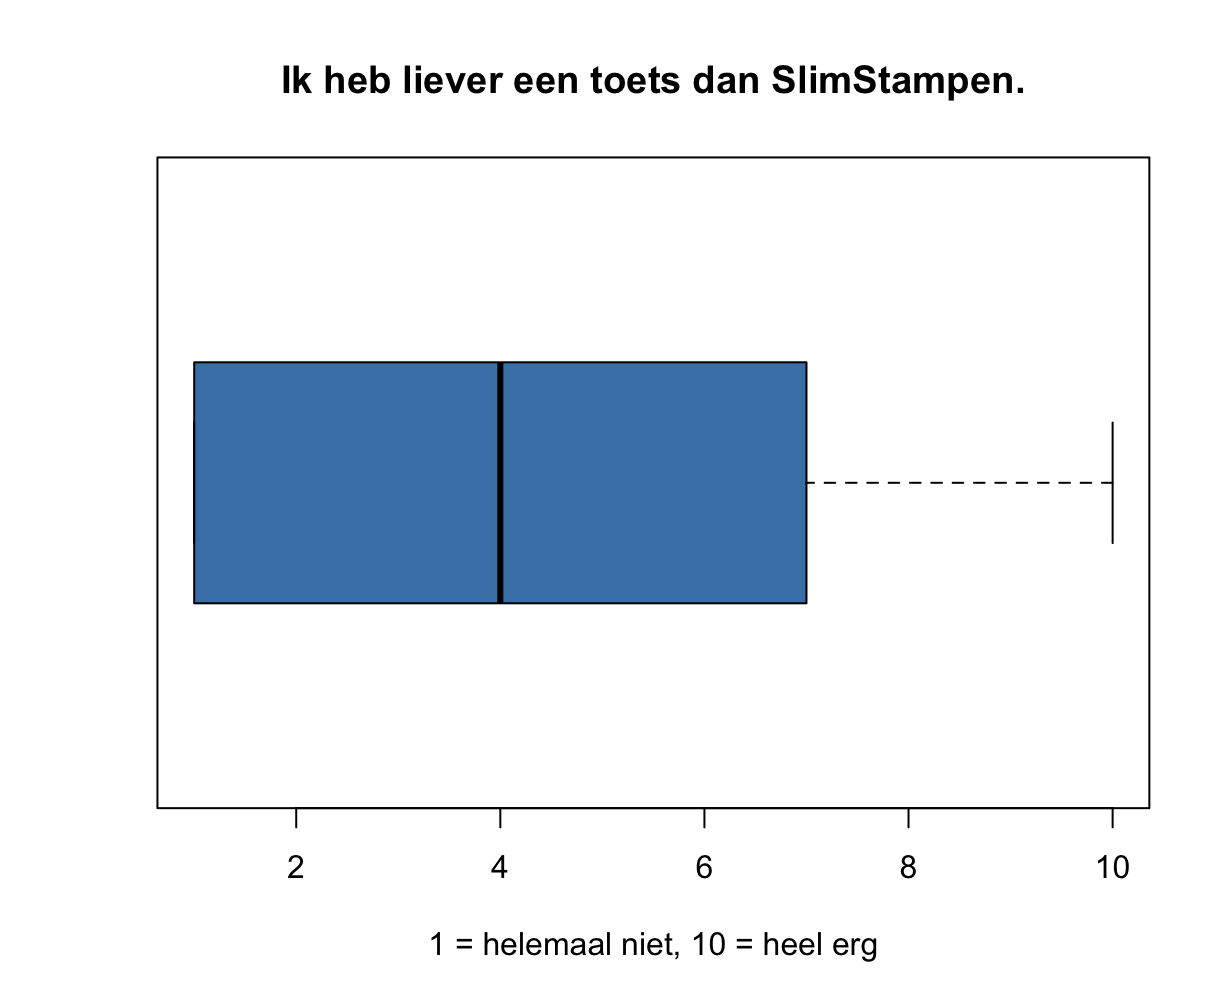
\includegraphics[width=65mm]{26-LieverToets.png} \\
        (a)  $\overline{X}$ = 7.841, N=283, NA = 54 & (b) $\overline{X}$ =  4.461, N=284, NA = 53 \\[6pt]
        \end{tabular}
        \caption{Evaluatie: toetsen of MemoryLab}
        \label{fig:evaluatie}
        \end{figure}

The first questions of the survey were about the student's knowledge of learning strategies. There were three questions where respondents could indicate on a scale of 1 to 10 how much they agreed with the statement. These three questions show that students are generally quite confident about their knowledge of learning strategies. As you can see in the three boxplots in figure ref*{fig:learning strategy}.

\begin{center}
    \begin{tabular}{|c|c|} 
    \hline
         keuzemogelijkheid & frequentie (N=337) \\
     \hline
     Op verschillende dagen de stof herhalen & 189 \\ 
     Mezelf laten overhoren door familie of vrienden & 170  \\ 
     Een overhoorprogramma op mijn computer of mobiel & 163 \\
     De feiten herhaald hardop lezen of overschrijven & 144  \\ 
     Andere & 36 \\
     \hline
    \end{tabular}
    \end{center}

The multiple-choice question ''To memorize factual knowledge, do I use these strategies?'' shows that students use multiple strategies. They could also fill in their own strategy and there were these different answers:
\emph{
'hanging a bill in places I frequent e.g. toilet and then repeating it when I am there', 'I write down the meanings of the facts somewhere', 'Making summaries', 'using MemoryLab', 'videos', 'chatGPT overhearing it', 'listening to music and going over it several times', 'Just normal' and 'mnomonics' }.
MemoryLab was mentioned several times separately when this use would have fit within one answer (namely, Using a crosstab program). More than half of the students use multiple strategies, with repeating and having rehearsals used most often. Many students are aware of the benefits of the spacing effect and retrieval practice.

My conclusion is that students generally think they know how to learn and memorize facts well. They use multiple strategies and are aware of the importance of spacing effect and retrieval practice. MemoryLab fits these strategies well. It is a retrieval program that students can use independently and that takes the spacing effect into account.

\subsection[Evaluation]{Evaluation of MemoryLab}
The evaluation of MemoryLab involved two closed-ended questions with scale of 1 to 10 and two open-ended questions. The questions were all about the repondents' assessment of the use of MemoryLab. The closed questions were asked in reverse for control purposes.
Figure ref*{fig:evaluation}(a) and (b) show that many students would like to see MemoryLab replace tests. The control question in (b) shows a slightly less negative score on whether they prefer tests than (a) has a positive score. The spread of responses is also higher in (b) than in (a). This may be due to the fact that all the other questions in the survey are positive. If they are not paying attention for a moment, the repondents may have given the wrong answer.

\begin{center}
    \begin{tabular}{|c|c|}
    \hline
         Bij welke vakken MemoryLab & frequentie (N=337) \\
     \hline
     Frans & 217 \\ 
     Duits & 152  \\ 
     aardrijkskunde & 129 \\
     Engels & 86  \\ 
     geschiedenis & 21 \\
     biologie & 9 \\
     wiskunde & 2 \\
     andere & 8 \\
     \hline
    \end{tabular}
    \end{center}
You can see that students at Metis Montessori Lyceum are already using MemoryLab in a lot of subjects. There are also subjects mentioned that I didn't know they teach with MemoryLab there as well. In the 'other' category, 'Greek' and 'physics' 'chemistry' were mentioned. These are subjects where we do not have lessons on our MemoryLab domain. It may very well be that students practice lessons on the general domain app.MemoryLab.nl for these subjects.

\begin{center}
    \begin{tabular}{|c|c|} 
    \hline
         Waarom gebruik je MemoryLab & frequentie (N=283) \\
     \hline
        verplicht/moet & 47 \\
        je krijgt punten op de toets & 18 \\
        handig/helpt & 128 \\
        neutraal & 63 \\
        nietszeggend, niet serieus & 27 \\
     \hline
    \end{tabular}
    \end{center}

The question ''Why do you use MemoryLab?'' was an open-ended question. Students were not directed in their answers at all. In part, this produced meaningless or neutral answers. After studying the various answers, I classified the answers into different categories. There is working with the program from a negative choice (it has to) and a positive choice (convenient or helps). There are students (47) who clearly do MemoryLab from an obligation. Furthermore, there are also students (18) who indicate that they do it from an incentive, they can earn extra points for the test by showing that they have practiced with MemoryLab. A number of students also give neutral answers, where there is no positive or negative choice, such as, for example, "to learn" or "for French. A number of answers were also given that were clearly not serious. The answers given show that most students use MemoryLab out of a positive choice. 'It is convenient', 'It helps with learning' and 'Because I had tried it once (we got extra points for that in French) and I had remembered the words very well, so now I use it more often'. The last answer indicates that the stimulus helped the experience. The student then made an independent positive choice to use it more often.

I can conclude that students use MemoryLab mainly because they find it convenient and it helps with learning. There are also students who do it because they have to, but that is a minority. The incentive of earning points for the test motivates students to use it. Replacing tests with MemoryLab is received positively by most students.

\subsection{Unexpected irregularity}
An irregularity in the use with MemoryLab in fourth grade emerged after the survey was administered. The learning data showed that some students achieved ''crowns'' far too quickly. Studying the learning data, I saw that students had a response time of exactly 500 milliseconds for each answer they gave. This time is virtually impossible for a human, and it is certainly out of the question that a human would achieve exactly this time for every answer. The suspicion was that a computer had answered, in other words there was ''a bot'' here.

The students who had created this bot were easily found, the code was on github, a site where programmers share their code and collaborate. Using a script, we discovered that 43 students had used the bot to retrieve crowns. The number of crowns obtained would be converted into a number and replace a test. With that, this was a serious problem. Why had these students chosen to do this?

This gave me an opportunity for unexpected and additional information for my research. Among the students who had used the bot, I sent out a questionnaire to find out what their motivations were for using the bot. Twelve students bothered to answer the questions comprehensively, which is 27.9 percent of bot users. This means that this information may not be very representative, but since it is substantively interesting and relevant, I decided to include it in this study anyway.

In the responses to why they used the bot (which you can read in Appendix A), you can see that students are generally not directly against MemoryLab, but more against the way it was deployed. This is valuable feedback. From the other responses (the questions are also in Appendix A), I read that students understand why MemoryLab works. They give a little more flexibility as an area for improvement. Eight of these students would prefer a test to MemoryLab, but four still prefer MemoryLab to a test. One student says he understands how MemoryLab works, but thinks that with a word list next to it, you can cheat by cheating. This is not entirely true, as it results in too long a reaction time. Thus, the student does not fully understand MemoryLab. I don't always completely agree with these students, but they have good points and we make education together. Teachers and students. We can and should do something with this. I will come back to that in the conclusion and recommendations.
\newpage
\section{Conclusion, reflection and recommendations}
The purpose of this study, based on a literature review and a survey of students, was to provide insight into the value of MemoryLab at a middle Montessori school. I translated the value into four key characteristics of Montessori education: the prepared environment, normalization, motivation and learning strategies. In addition, I used a student survey to evaluate the use of MemoryLab.

The prepared environment is an important feature of Montessori education. MemoryLab is a digital learning environment that helps students learn factual knowledge. The survey shows that students are positive about the clarity and clarity of MemoryLab. They know what to do and can use it independently. This fits well with Maria Montessori's idea of the prepared environment.

Learner normalization is another important feature of Montessori education. Normalization touches on the learner's task acceptance. The survey shows that MemoryLab helps with concentration and students get to work focused. They are not easily distracted and feel more confident about their abilities. This fits well with what Maria Montessori saw as normalization.

Student motivation is a third important characteristic of Montessori education. The survey shows that MemoryLab has a positive impact on learner motivation. Students like that they have more autonomy and start learning earlier for a test. All of this leads to better grades.

Learning strategies are a fourth important feature of Montessori education. The survey shows that students generally think they know how to learn and memorize factual knowledge well. They use multiple strategies and are aware of the importance of the spacing effect and retrieval practice. MemoryLab fits well into these strategies. It is a retrieval program that students can use independently and that takes into account the spacing effect.

The evaluation of MemoryLab with the students shows that they are generally positive about using MemoryLab. They find it convenient and it helps with learning. Most students would like to see MemoryLab replace tests. This fits well with the idea of independent work and free choice in Montessori education.

The answer to the research question is that MemoryLab is a valuable addition to Montessori education. It contributes to the student's prepared environment, normalization, motivation and learning strategies. It is a digital learning environment that helps learners learn factual knowledge and fits well with the principles of Montessori education. With that, this research contributes to the further development of montessori education and I can use this research to substantiate that MemoryLab is a valuable addition to montessori education in conversation with my colleagues, the school administration and the developers of MemoryLab.

During my literature review, I delved into the meaning and importance of standardization. In doing so, I went back to the ideas of a number of Enlightenment philosophers. I discovered many ideas of Montessori education in these philosophers. Maria Montessori, in my opinion, could have given more credit to them here. I found the search for the background of her ideas valuable. It gave me more depth and confidence in my role as a teacher. I find the missing references in Maria Montessori's books a miss. Perhaps one explanation is that she considered herself a scientist and not a philosopher. She manifested herself as an empiricist by emphasizing observation and less as a rationalist, when in my opinion she was indeed a rationalist as well.

An important finding for me is that three characteristics I have described are significantly related. The prepared environment is important for normalization and from normalization flows motivation. This again fits with Maria Montessori's idea of cosmic education. Everything is interrelated.

I find the tension between freedom and discipline in education fascinating. This was a focus for me during this research. I now understand much better what is meant by these concepts, in relation to Maria Montessori's \emph{freedom in bondage}. To many outsiders, Montessori education stands for freedom. This is a strong misconception. Discipline is an important element within Montessori education. Not imposed (authoritarian) discipline, but self-chosen discipline. Only with self-chosen discipline can you experience true freedom, because in a society there are always rules that you must follow. These rules can give you a sense of limitation if you don't accept them. So only if you accept these rules can you feel free. Some students react indignantly when faced with a test or a school rule, others feel free in their choices. The self-chosen deep concentration when you work, the working without the teacher telling you to work. This is the discipline or normalization that Maria Montessori is looking for in the student. From this normalization, higher motivation for school usually follows.  

Data from the survey show that students are positive about MemoryLab as a Montessori material. The self-scheduling of time, the clarity of the material and the possible replacement of tests with MemoryLab is highly appreciated. I myself also see MemoryLab as a learning tool for teaching learning strategies, such as repetition and retrieval, this is not seen by all students, but many students do see this value of MemoryLab. Many students are already familiar with these learning strategies. Students report getting into a concentration well when using MemoryLab. They are not easily distracted when working on this task. Working with MemoryLab allows students to experience a little more autonomy.

MemoryLab helps with motivation for students, as evidenced by the fact that they enjoy learning with MemoryLab more than having to learn rows on their own. Learning with MemoryLab gives a positive feeling afterwards. Students like being able to manage more of their own time. They feel more confident about their ability in school because of MemoryLab and feel that they are now getting higher grades. MemoryLab creates a sense of competence in many students.

In the subjects French, German, geography and English, MemoryLab is already widely used at our school. Students look forward to the possibility that MemoryLab can replace a test. Seventy-five percent of the students are positive to very positive about this. A small number of students are not. And we need to do more research on that.

In the fourth grade English course this year, a test was actually replaced by MemoryLab. You would think given the results of my research that this would be welcomed. This is not the case with some students. Replacing the test with this learning algorithm prompted some students to develop and use a bot. The computer obtained the required crowns instead of the students. Where did this behavior come from? This is what I asked the students who used the bot about. The results were illuminating. Of the students who used the bot, most were not negative about MemoryLab, but about the way it was deployed.

This is valuable information that I also shared with Utrecht University, because this requires more research. I thought we were giving students more autonomy by not giving a test on a date we set. This was not perceived that way. The students felt forced by us to learn all the words. They indicated that they could already do English and would just take the test. They would already get a passing grade for this without learning too much. With MemoryLab, you don't get a crown until you know 100 percent of the words. This requires a completely different approach. Teachers need to think carefully about which words they really think students should know. What percentage is sufficient? This is an important consideration.

We must also remember that the students who used the bot are a small group. Most students simply used MemoryLab as it was intended and as the teachers intended. Then you come to an important question: can we accommodate all the students' needs? The fact that students who used the bot often indicated that it was used correctly in German and not in English indicates that there is a difference in how MemoryLab is used. This is the next major area of concern.

I have made several recommendations in this study for the school and the developers of MemoryLab. I think it is important for the school to think carefully about the way MemoryLab is deployed. Points to consider are:
\begin{itemize}
    \item Hoeveel procent van de feiten moet een leerling beheersen om voldoende kennis te hebben volgens de docenten?
    \item Hoe zetten we MemoryLab in, moet het een toets vervangen of is het een hulpmiddel voor de leerling?
    \item Alle docenten op de hoogte stellen van mijn bevindingen en samen met hen kijken naar de manier waarop MemoryLab wordt ingezet.
    \item Wat is essentiele feitelijke kennis en wat is extra kennis? Alleen de essentiele kennis moet in MemoryLab.
\end{itemize}

I now have the role of MemoryLab coordinator within the entire MSA. Teachers at the various schools are finding me better and better and are already asking about results of my research. In this research, I focused primarily on the students. I think it is important to also involve teachers in the evaluation of MemoryLab. They can provide valuable feedback on the use of MemoryLab in the classroom. I think it would be good to set up a working group with teachers who use MemoryLab in the classroom. They can work with me to look at the survey results and the recommendations I have made. That way we can work together to improve the use of MemoryLab in the classroom.

With MemoryLab and Utrecht University, the MSA has funding for two more years to conduct further research on the use of a learning algorithm in secondary education. Some of the above concerns will be addressed in this. I hope to play another important role in this.
\newpage
\appendix
\section{Appendix}
\emph{Why did you decide to use the bot?}

\begin{enumerate}
    \item The English glossary of MemoryLab took a very long time to create and it felt more like a rotten job than something I learned from. I decided to use the bot to save myself the time and effort for something that seemed unnecessary to me.
    \item First, let me say that I only used the bot for English, not for German because with German it works well. you learn words and those words come along with grammar in the test. In English, on the other hand, MemoryLab is a separate grade which I find weird.
    \item I wanted to try it out and I don't think our class even had to do smart word processing.
    \item It was too many assignments for English.
    \item It was too repetitive, repeated itself too often. More often than it should have.
    \item I used the bot purely for english, where you have to 'learn' 12 word lists dutch-english and english-dutch to not get a 1 on your final report. the only downside is that these lists are not always translated correctly so it is often difficult to make the lists even if i know all the words well and can work them correctly into a sentence.
    \item  I sincerely think MemoryLab is a good system. The reason why I used the bot is because English was a lot. In some subjects it is well done like German and in some subjects it is very poorly done like English. In German, the lists of MemoryLab are optional, but you get bonus points if you make them. I think this is a win win situation because so if you are good at German you don't have to do the lists and if you are bad at German I would make the lists so you learn the words better and so you can get the bonus points. With English it is compulsory, because of this the people who are good at English still have to put a lot of time into it, which ends up making you very demotivated. What English also does is instead of giving 12 lists for the 12 units it gives you 24 lists, 12 for NL-ENG and 12 for ENG-NL. This makes you do twice as much work so it ends up feeling like you're working indefinitely. A lot of students found this too much work. That is also the reason why [name removed due to privacy - MM] and [name removed due to privacy - MM] made that bot. I think it would be better if the English lists were the same as the German lists. Other than that, I think using MemoryLab is a great alternative to large vocabulary tests and a convenient way for mashing words, with exceptions for how bad the English lists are.
    \item 1. Because I didn't feel like ''learning'' all those hundreds of words of English. I already knew all those words of English.
     2. Even if I didn't know the words, I like not being forced to type the same thing two hundred times for a grade. It feels like brain-dead typing, especially so if you already know the words. So I would like it better if the word lists (like in German) were as an optional tool for words on tests.‖
    3. Writing a program with python and HTTP seemed many times more fun than that typing.â
    4. It's even better to learn words with sentences anyway instead of testing the words individually, then you still don't know how it would fit into a sentence in another language (if you really don't know that language very well yet).''►
    \item ''I already know the words, I've been speaking English daily for years. I find that for me it's a waste of time.‖
    \item No point in cramming for English 16-30 hours of words I already know. \\
    \item I had used it for english because we got 24 lists at once there and that takes quite a bit of time.â
    \item Because using MemoryLab takes a very long time, the lists are not practical (words that are also correct are not computed correctly) and the system is not pleasant to use. With a bot, it's faster while I can still learn.â
\end{enumerate}

Other questions for these students:_____.
\begin{enumerate}
\item I'd rather have a test than MemoryLab....
\item I think I understand why the use of MemoryLab works?
\item If I read this explanation, I understand more about the use of MemoryLab
     https://www.memorylab.nl/wetenschap/ and make me more positive about using MemoryLab?
     \item What should be improved about MemoryLab so that I do enjoy using it?
     \item This is what I want to say....
\end{enumerate}

\newpage
\bibliographystyle{apacite} 
\bibliography{bibliography}

\end{document}
